\documentclass[a4paper,ngerman]{scrartcl}

\usepackage[utf8]{inputenc}

\usepackage[ngerman]{babel}

\usepackage{amsmath,amsthm,amssymb,stmaryrd,color,graphicx}
\usepackage{bussproofs}
\usepackage{array}
\usepackage{comment}

\usepackage[protrusion=true,expansion=true]{microtype}

\usepackage{lmodern}
\usepackage{tabto}

\usepackage[natbib=true,style=numeric]{biblatex}
\usepackage[babel]{csquotes}
\bibliography{literatur}

\usepackage[all]{xy}

\usepackage{hyperref}

\setlength\parskip{\medskipamount}
\setlength\parindent{0pt}

\theoremstyle{definition}
\newtheorem{defn}{Definition}[section]
\newtheorem{bsp}[defn]{Beispiel}

\theoremstyle{plain}

\newtheorem{prop}[defn]{Proposition}
\newtheorem{motto}[defn]{Motto}
\newtheorem{ueberlegung}[defn]{Überlegung}
\newtheorem{lemma}[defn]{Lemma}
\newtheorem{kor}[defn]{Korollar}
\newtheorem{hilfsaussage}[defn]{Hilfsaussage}
\newtheorem{satz}[defn]{Satz}

\theoremstyle{remark}
\newtheorem{bem}[defn]{Bemerkung}
\newtheorem{aufg}[defn]{Aufgabe}

\clubpenalty=10000
\widowpenalty=10000
\displaywidowpenalty=10000

\newcommand{\xra}[1]{\xrightarrow{#1}}
\newcommand{\lra}{\longrightarrow}
\newcommand{\lhra}{\ensuremath{\lhook\joinrel\relbar\joinrel\rightarrow}}
\newcommand{\thlra}{\relbar\joinrel\twoheadrightarrow}

\newcommand{\ZZ}{\mathbb{Z}}
\newcommand{\QQ}{\mathbb{Q}}
\newcommand{\RR}{\mathbb{R}}
\newcommand{\NN}{\mathbb{N}}
\newcommand{\PP}{\mathbb{P}}
\newcommand{\I}{\mathcal{I}}
\newcommand{\J}{\mathcal{J}}
\newcommand{\C}{\mathcal{C}}
\newcommand{\D}{\mathcal{D}}
\newcommand{\E}{\mathcal{E}}
\renewcommand{\I}{\mathcal{I}}
\renewcommand{\P}{\mathcal{P}}
\renewcommand{\O}{\mathcal{O}}
\newcommand{\Hom}{\mathrm{Hom}}
\newcommand{\ev}{\mathrm{ev}}
\newcommand{\id}{\mathrm{id}}
\newcommand{\Id}{\mathrm{Id}}
\newcommand{\freist}{\underline{\ \ }}
\DeclareMathOperator{\colim}{colim}
\DeclareMathOperator{\Ob}{Ob}
\DeclareMathOperator{\ggT}{ggT}
\newcommand{\op}{\mathrm{op}}
\newcommand{\Set}{\mathrm{Set}}
\newcommand{\Grp}{\mathrm{Grp}}
\newcommand{\Vect}[1]{{#1\text{-}\mathrm{Vect}}}
\newcommand{\AbGrp}{\mathrm{AbGrp}}
\newcommand{\Ring}{\mathrm{Ring}}
\newcommand{\Cat}{\mathrm{Cat}}
\newcommand{\Funct}{\mathrm{Funct}}
\newcommand{\Eins}{\mathbf{1}}
\newcommand{\Man}{\mathrm{Man}}
\newcommand{\Top}{\mathrm{Top}}
\newcommand{\seq}[1]{\mathrel{\vdash\!\!\!_{#1}}}

\newcommand{\XXX}[1]{\textcolor{red}{#1}}

\renewcommand*\theenumi{\alph{enumi}}
\renewcommand{\labelenumi}{\theenumi)}

\newcommand\subsubsubsection[1]{\subsubsection*{#1}}
\definecolor{grey}{rgb}{0.7,0.7,0.7}

\setcounter{tocdepth}{2}

\newenvironment{indentblock}{%
  \list{}{\leftmargin\leftmargin}%
  \item\relax
}{%
  \endlist
}

%\newarrow{Equals}=====

%\usepackage{geometry}
%\geometry{tmargin=2cm,bmargin=4cm,lmargin=3cm,rmargin=3cm}

\begin{document}

\vspace*{2em}%
\begin{center}%
  \vskip 1em
  {\LARGE Pizzaseminar zur Kategorientheorie}
  \vskip 1.5em%
  {\large
   \lineskip .5em%
    \begin{tabular}[t]{c}%
      \today
    \end{tabular}\par}%
    \vskip 1em%
\end{center}\par
\par\vskip 1.5em

\begin{center}\emph{in Entstehung befindlich} \\ \ \\
\TeX{}er: Tim Baumann, Ingo Blechschmidt, Justin Gassner, Lukas Graf, Maximilian~Huber, Matthias Hutzler\end{center}

\tableofcontents

\documentclass[12pt,utf8,notheorems,compress]{beamer}

\usepackage[ngerman]{babel}

\usepackage{amsmath,amssymb}
%\usepackage[framed,amsmath,thmmarks,hyperref]{ntheorem}

%\usepackage[small,nohug]{diagrams}
%\diagramstyle[labelstyle=\scriptstyle]

%\usepackage[protrusion=true,expansion=false]{microtype}

%\usepackage{lmodern}
\usepackage{tabto}
\usepackage{tikz}
\usepackage{array}
\usepackage[all]{xy}

%\usepackage[natbib=true,style=numeric]{biblatex}
%\usepackage[babel]{csquotes}
%\bibliography{lit}

%\usepackage{hyperref}

\setlength\parskip{\medskipamount}
\setlength\parindent{0pt}

%\theoremseparator{:}
\theoremstyle{plain}  %nonumberplain
%\newtheorem{beh}{Behauptung}
\newtheorem{proposition}{Proposition}
\newtheorem{corollary}{Korollar}
\newtheorem{theorem}{Satz}
\theoremstyle{definition}
\newtheorem{definition}{Definition}
%\newtheorem{kor}{Korollar}
%\newtheorem{satz}{Satz}
%\newtheorem{lemma}{Lemma}
%\newtheorem{hilfsaussage}{Hilfsaussage}
%\theorembodyfont{\normalfont}
\newtheorem{axiom}{Axiom}
%\newtheorem{defnprop}{Definition/Proposition}
%\newtheorem{bem}{Bemerkung}
%\newtheorem{bsp}{Beispiel}
%\theoremsymbol{\ensuremath{\openbox}}
%\newtheorem{proof}{Beweis}
%\newtheorem{defn}{Definition}

\newcommand{\lra}{\longrightarrow}
\newcommand{\lhra}{\ensuremath{\lhook\joinrel\relbar\joinrel\rightarrow}}
\newcommand{\thlra}{\relbar\joinrel\twoheadrightarrow}

\newcommand{\Z}{\mathbb{Z}}
\renewcommand{\C}{\mathcal{C}}
\newcommand{\N}{\mathbb{N}}
\newcommand{\R}{\mathbb{R}}
\newcommand{\Hom}{\mathrm{Hom}}
\newcommand{\id}{\mathrm{id}}
\newcommand{\Aut}[1]{\operatorname{Aut}(#1)}
\newcommand{\GL}[1]{\operatorname{GL}(#1)}
\newcommand{\freist}{\_{}\_{}}
\newcommand{\Set}{\mathrm{Set}}
\newcommand{\Grp}{\mathrm{Grp}}
\newcommand{\Vect}{\mathrm{Vect}}

\def\longleadsto{\mathrel{-}\joinrel\leadsto}
\DeclareMathOperator{\ggT}{ggT}
\DeclareMathOperator{\Ob}{Ob}
\newcommand{\op}{\mathrm{op}}

\title{Was sind und was sollen Kategorien?}
\author[Pizzaseminar in Mathematik]{%
  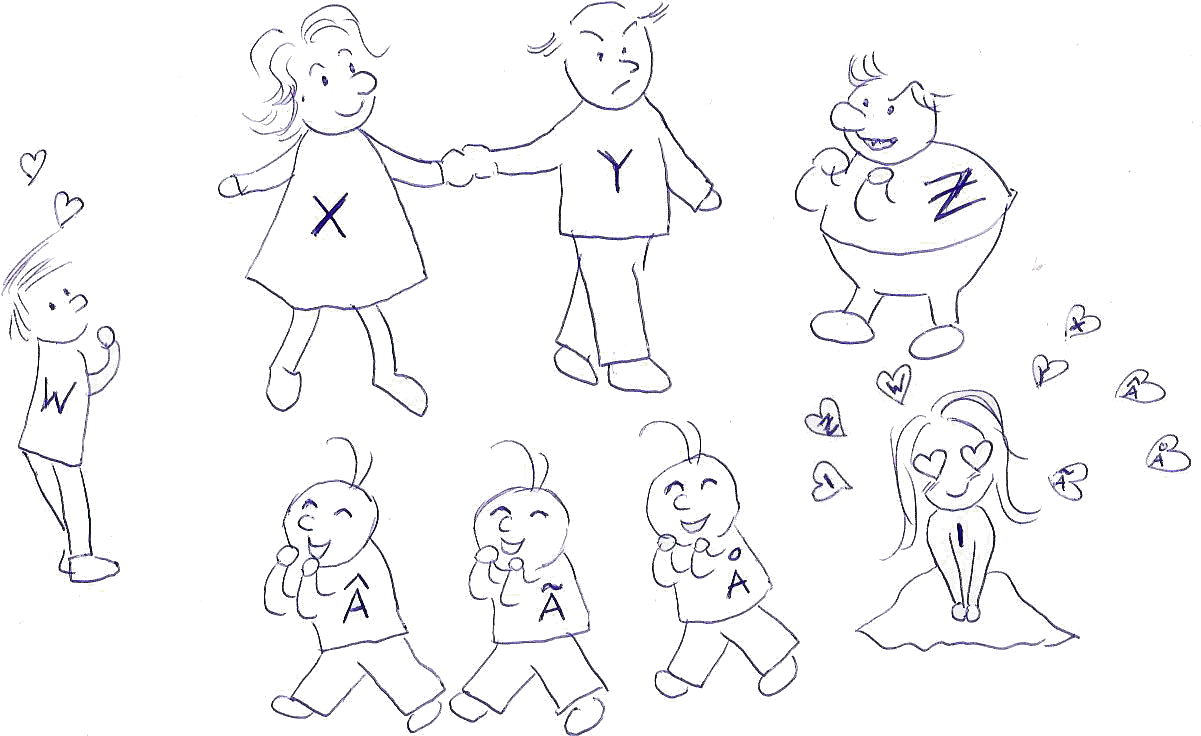
\includegraphics[scale=0.4]{relationen.png}}
%Ingo Blechschmidt \\ mit Illustrationen von Carina Willbold}
%\institute{Pizzaseminar in Mathematik}
\date{27. Februar 2013}

%\usetheme{Warsaw}  %Warsaw, Berkeley?
\usetheme{Warsaw}
\useoutertheme{split}
\usecolortheme{seahorse}
\usefonttheme{serif}
\usepackage{palatino}
\useinnertheme{rectangles}
%\usepackage{bookman}
%\setbeamercovered{transparent}

\setbeamertemplate{navigation symbols}{}
%\setbeamertemplate{footline}{}
%\setbeamertemplate{headline}{}

%\beamertemplateboldcenterframetitle
%\setbeamerfont{frametitle}{size={\Large}}

\newcommand*\oldmacro{}%
\let\oldmacro\insertshorttitle%
\renewcommand*\insertshorttitle{%
  \oldmacro\hfill\insertframenumber\,/\,\inserttotalframenumber\hfill}

\newenvironment{changemargin}[2]{%
  \begin{list}{}{%
    \setlength{\topsep}{0pt}%
    \setlength{\leftmargin}{#1}%
    \setlength{\rightmargin}{#2}%
    \setlength{\listparindent}{\parindent}%
    \setlength{\itemindent}{\parindent}%
    \setlength{\parsep}{\parskip}%
  }%
  \item[]}{\end{list}}

\newcommand{\slogan}[1]{%
  \begin{center}%
    \setlength{\fboxrule}{2pt}%
    \setlength{\fboxsep}{-3pt}%
    {\usebeamercolor[fg]{item}\fbox{\usebeamercolor[fg]{normal
    text}\parbox{0.9\textwidth}{\begin{center}#1\end{center}}}}%
  \end{center}%
}

\newcommand{\hil}[1]{{\usebeamercolor[fg]{item}{#1}}}

\begin{document}

\setbeameroption{show notes}
\setbeamertemplate{note page}[plain]

\frame{\titlepage}
%\frame[t]{\frametitle{Gliederung}\begin{minipage}{\textwidth}\begin{small}\tableofcontents\end{small}\end{minipage}}
\frame[t]{\frametitle{Gliederung}\tableofcontents}

\section[Motivation]{Motivation: Beispiele für kategorielles Verständnis}

\subsection{Produkte}
\frame[t]{\frametitle{Produkte in Kategorien I}
  \begin{itemize}
    \item Kartesisches Produkt von Mengen: $X \times Y$
    \item Kartesisches Produkt von Vektorräumen: $V \times W$
    \item Kartesisches Produkt von Gruppen: $G \times H$
    \item Kartesisches Produkt von Garben: $\mathcal{F} \times \mathcal{G}$
    \item Kartesisches Produkt von Vektorbündeln: $\mathcal{E} \times \mathcal{F}$
    \item Minimum von Zahlen: $\min\{n,m\}$
    \item Größter gemeinsamer Teiler von Zahlen: $\ggT(n,m)$
    \item Paartyp in Programmiersprachen: \texttt{(a,b)}
    \item Mutterknoten zweier Knoten in einem Graph
  \end{itemize}

  \slogan{%
    All dies sind Spezialfälle des allgemeinen \\ \emph{kategoriellen Produkts}.
  }

  \begin{tikzpicture}[remember picture,overlay]  
    \node [xshift=-1cm,yshift=-8.5cm] at (current page.north east)
      {
\includegraphics[scale=0.4]{produkt.png}};
  \end{tikzpicture}
}

\frame[t]{\frametitle{Produkte in Kategorien II}
  \begin{align*}
    X \times (Y \times Z) &\cong (X \times Y) \times Z \\
    U \times (V \times W) &\cong (U \times V) \times W \\
    \min\{m,\min\{n,p\}\} &= \min\{\min\{m,n\},p\} \\
    \ggT(m,\ggT(n,p)) &= \ggT(\ggT(m,n),p)
  \end{align*}

  \slogan{%
    All dies sind Spezialfälle der allgemeinen \\ \emph{Assoziativität} des kategoriellen Produkts.
  }

  \begin{tikzpicture}[remember picture,overlay]  
    \node [xshift=-1cm,yshift=-7.5cm] at (current page.north east)
      {
\includegraphics[scale=0.4]{produkt.png}};
  \end{tikzpicture}
}

\subsection{Isomorphismen}
\frame[t]{\frametitle{Isomorphismen in Kategorien}
  \begin{itemize}
    \item Zwei Mengen $X,Y$ \tabto{4.63cm} können gleichmächtig sein.
    \item Zwei Vektorräume $V,W$ \tabto{4.63cm} können isomorph sein.
    \item Zwei Gruppen $G,H$ \tabto{4.63cm} können isomorph sein.
    \item Zwei top. Räume $X,Y$ \tabto{4.63cm} können homöomorph sein.
    \item Zwei Zahlen $n,m$ \tabto{4.63cm} können gleich sein.
    \item Zwei Typen \texttt{a}, \texttt{b} \tabto{4.63cm} können sich verlustfrei ineinander umwandeln lassen.
  \end{itemize}

  \slogan{%
    All dies sind Spezialfälle des allgemeinen \\ \emph{kategoriellen
    Isomorphiekonzepts}.
  }

  \begin{tikzpicture}[remember picture,overlay]  
    \node [xshift=-1.1cm,yshift=-8.0cm] at (current page.north east)
      {
\includegraphics[scale=0.4]{isomorphie.png}};
  \end{tikzpicture}
}

\subsection{Dualität}
\frame[t]{\frametitle{Dualität}
  \vspace{-0.5em}
  \begin{center}
    \setlength{\extrarowheight}{0.3em}
    \begin{tabular}{r|l}
      $f \circ g$ & $g \circ f$ \\
      $\leq$ & $\geq$ \\
      injektiv & surjektiv \\
      $\{\star\}$ & $\emptyset$ \\
      $\times$ & $\coprod$ \\
      ggT & kgV \\
      $\cap$ & $\cup$ \\
      Teilmenge & Faktormenge
    \end{tabular}
  \end{center}

  \slogan{%
    All dies sind Spezialfälle eines allgemeinen \\
    \emph{kategoriellen Dualitätsprinzips}.
  }

  \begin{tikzpicture}[remember picture,overlay]  
    \node [xshift=-1cm,yshift=-7.5cm] at (current page.north east)
      {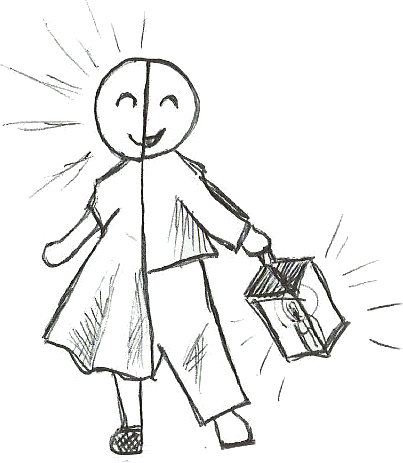
\includegraphics[scale=0.4]{dualitaet.png}};
  \end{tikzpicture}
}


\section{Grundlagen}

\subsection[Def.]{Definition des Kategorienbegriffs}
\frame[t,shrink=10]{\frametitle{Kategorien}%
  \begin{tikzpicture}[remember picture,overlay]
    \node [xshift=1cm,yshift=-2cm] at (current page.north east)
      {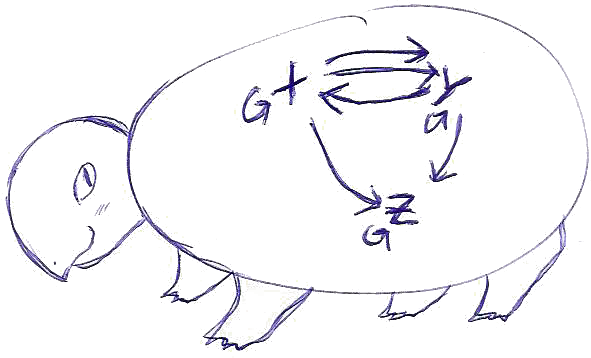
\includegraphics[scale=0.4]{kategorie.png}};
  \end{tikzpicture}%
  %\begin{definition}
    \textbf{Definition:} Eine Kategorie~$\C$ besteht aus
    \begin{enumerate}
      \item einer Klasse von \emph{Objekten} $\Ob \C$,
      \item zu je zwei Objekten $X,Y \in \Ob \C$ einer Klasse $\Hom_\C(X,Y)$ von
      \emph{Morphismen} zwischen ihnen und
      \item einer Kompositionsvorschrift:
      \begin{align*}
        \text{zu }\ & f \in \Hom_\C(X,Y) &
        \text{zu }\ & f : X \to Y \\
        \text{und }\ & g\in\Hom_\C(Y,Z) &
        \text{und }\ & g : Y \to Z \\
        \text{habe }\ & g\circ f\in\Hom_\C(X,Z), &
        \text{habe }\ & g\circ f : X \to Z,
      \end{align*}
    \end{enumerate}
    sodass
    \begin{enumerate}
      \item die Komposition $\circ$ assoziativ ist und
      \item es zu jedem $X \in \Ob\C$ einen \emph{Identitätsmorphismus} $\id_X
      \in \Hom_\C(X,X)$ mit
      \[ f \circ \id_X = f, \quad \id_X \circ g = g \]
      für alle Morphismen $f,g$ gibt.
    \end{enumerate}
  %\end{definition}
}

\note{
  \begin{itemize}
    \item Die Morphismen müssen nicht unbedingt Abbildungen
    sein. Die Schreibweise "`$f:X \to Y$"' missbraucht also Notation.
    \item Archetypisches Beispiel ist $\Set$, die Kategorie der Mengen und Abbildungen:
    \begin{align*}
      \Ob \Set &:= \{ M \,|\, \text{$M$ ist eine Menge} \} \\
      \Hom_\Set(X,Y) &:= \{ f:X \to Y \,|\, \text{$f$ ist eine Abbildung} \}
    \end{align*}
    \item Die meisten Teilgebiete der Mathematik studieren jeweils eine bestimmte
    Kategorie: Gruppentheoretiker beschäftigen sich etwa mit der Kategorie
    $\Grp$ der Gruppen und Gruppenhomomorphismen:
    \begin{align*}
      \Ob \Grp &:= \text{Klasse aller Gruppen} \\
      \Hom_\Grp(G,H) &:= \{ f:G \to H \,|\, \text{$f$ ist ein Gruppenhomo} \}
    \end{align*}
  \end{itemize}
}

\note{
  \begin{itemize}
    \item Es gibt aber auch wesentlich kleinere Kategorien. Etwa kann man aus
    jeder Partialordnung~$(P,\preceq)$ eine Kategorie~$\C$ basteln:
    \begin{align*}
      \Ob \C &:= P \\
      \Hom_\C(x,y) &:= \begin{cases}
        \text{einelementige Menge}, & \text{falls $x \preceq y$,} \\
        \text{leere Menge}, & \text{sonst}
      \end{cases}
    \end{align*}

    \item Auch sind gewisse endliche Kategorien bedeutsam, etwa die durch
    folgende Skizze gegebene:

    \[ \xymatrix{
      & \bullet \ar[d] \ar@(ur,ul) \\
      \bullet \ar[r] \ar@(ul,dl) & \bullet \ar@(dr,ur)
    } \]
  \end{itemize}
}

\note{
  Gleichungen zwischen Morphismen schreibt man gerne als kommutative
  Diagramme:
  \[ h = g \circ f
    \quad\quad\Longleftrightarrow:\quad\quad
    \vcenter{\xymatrix{
      X \ar[rr]^f \ar[ddr]_h & & Y \ar[ddl]^g \\
      & \% \\
      & Z
    }}
  \]
}


\frame[t]{\frametitle{Fundamentales Motto}
  \slogan{%
    Kategorientheorie stellt \emph{Beziehungen zwischen Objekten} statt
    etwaiger innerer Struktur in den Vordergrund.}

  \begin{center}
    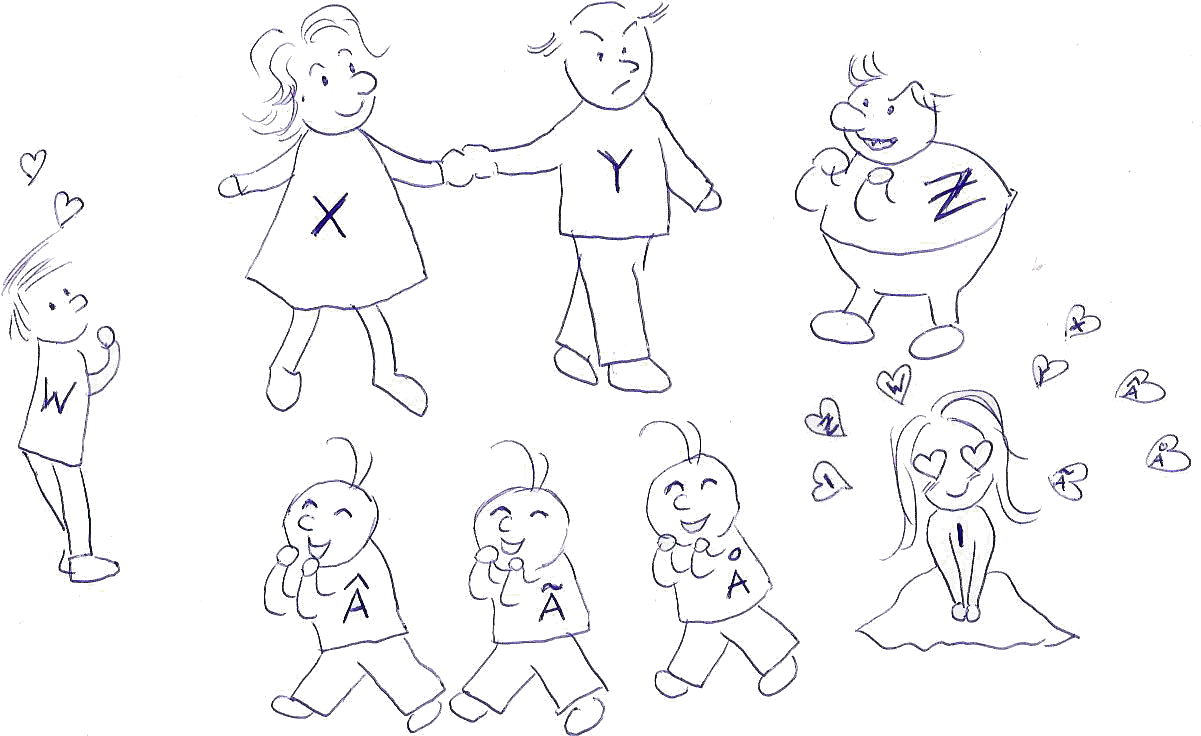
\includegraphics[scale=0.3]{relationen.png}
  \end{center}
}

\subsection[Initiale u. terminale Obj.]{Initiale und terminale Objekte}
\frame[t]{\frametitle{Initiale und terminale Objekte}
  \textbf{Definition:} Ein Objekt~$X$ einer Kategorie~$\C$ heißt genau dann
  \begin{itemize}
    \item \emph{initial}, wenn
      \[ \forall Y \in \Ob \C{:}\ \exists! f : X \to Y. \]
    \item \emph{terminal}, wenn
      \[ \forall Y \in \Ob \C{:}\ \exists! f : Y \to X. \]
  \end{itemize}

  \vfill
  \only<1>{\textbf{Frage:} Was ist ein terminales Objekt in~$\Set$?}
  \only<2>{%
    In $\Set$: \tabto{2.15cm} $\emptyset$ initial, $\{\star\}$ terminal.

    In $\R{-}\Vect$: \tabto{2.15cm} $\R^0$ initial und terminal.}
}

\subsection[Monos und Epis]{Mono- und Epimorphismen}
\frame[t]{\frametitle{Mono- und Epimorphismen}
  \textbf{Definition:}
  Ein Morphismus $f:X \to Y$ einer Kategorie~$\C$ heißt genau dann
  \begin{itemize}
    \item \emph{Monomorphismus}, \tabto{3.35cm}wenn für alle Objekte~$A \in \Ob \C$ \\
    \tabto{3.35cm}und $p,q:A \to X$ gilt:
    \[ f \circ p = f \circ q \quad\Longrightarrow\quad p = q. \]
    \item \emph{Epimorphismus}, \tabto{3.35cm}wenn für alle Objekte~$A \in \Ob \C$ \\
    \tabto{3.35cm}und $p,q:Y \to A$ gilt:
    \[ p \circ f = q \circ f \quad\Longrightarrow\quad p = q. \]
  \end{itemize}

  \textbf{Beobachtung} in $\Set$, $\Grp$ und $\R{-}\Vect$:
  \begin{align*}
    \text{$f$ Mono} &\Longleftrightarrow \text{$f$ injektiv.} \\
    \text{$f$ Epi} &\Longleftrightarrow \text{$f$ surjektiv.}
  \end{align*}
}

\subsection[Duale Kat.]{Die duale Kategorie einer Kategorie}
\frame[t]{\frametitle{Duale Kategorie}%
  \begin{itemize}
    \item \textbf{Definition:} Zu jeder Kategorie~$\C$ gibt es eine zugehörige
    \emph{duale Kategorie} $\C^\op$:
    \begin{align*}
      \Ob \C^\op &:= \Ob \C \\
      \Hom_{\C^\op}(X,Y) &:= \Hom_\C(Y,X)
    \end{align*}
    \item \textbf{Beispiel:} $\quad$ $X$ in $\C^\op$ initial
    $\quad\Longleftrightarrow\quad$ $X$ in $\C$ terminal
    \item \textbf{Beispiel:} $\quad$ $f$ in $\C^\op$ Mono $\quad\Longleftrightarrow\quad$ $f$ in $\C$ Epi
    \item \textbf{Nichttriviale Frage:} Wie kann man in konkreten
    Fällen~$\C^\op$ explizit (inhaltlich) beschreiben?
  \end{itemize}

  \begin{center}
    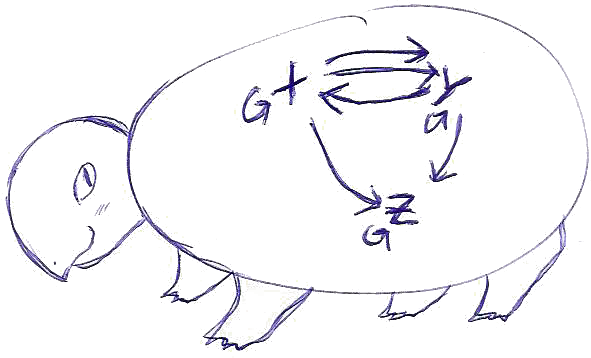
\includegraphics[scale=0.3]{kategorie.png}\quad
    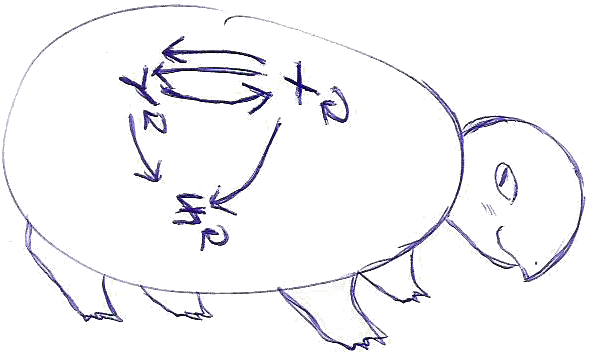
\includegraphics[scale=0.3]{kategorie-dual.png}
  \end{center}
}

\section{Anwendungen}
\frame[t]{\frametitle{Anwendungen}%
  \begin{itemize}
    \item Kategorientheorie liefert einen Leitfaden, \\ um richtige Definitionen
    zu formulieren.

    \item Triviales wird \emph{trivialerweise} trivial: \\
    \hil{Allgemeiner abstrakter Nonsens.}

    \item Konzeptionelle Vereinheitlichung: Viele Konstruktionen in der
    Mathematik sind Spezialfälle von allgemeinen kategoriellen: \\
    \hil{Limiten, Kolimiten, adjungierte Funktoren}

    \item Forschungsprogramm der Kategorifizierung,
          um tiefere Gründe für Altbekanntes zu finden.
    \item siehe Bonusthemen!
  \end{itemize}

  \begin{tikzpicture}[remember picture,overlay]
    \node [xshift=-1cm,yshift=-3cm] at (current page.north east)
      {
\includegraphics[scale=0.3]{nonsens.png}};
  \end{tikzpicture}%
}

% XXX: "All dies" vs. "Alle diese"

\end{document}

\section[Produkte und Koprodukte]{Produkte und Koprodukte \hfill \small
Matthias Hutzler}

\begin{defn}Seien~$X$, $Y$ Objekte einer Kategorie~$\C$. Dann besteht ein
\emph{Produkt} von~$X$ und~$Y$ aus
\begin{enumerate}
\item einem Objekt~$P \in \Ob \C$ und
\item Morphismen $\pi_X : P \to X$, $\pi_Y : P \to Y$,
\end{enumerate}
sodass für jedes andere \emph{Möchtegern-Produkt}, also
\begin{enumerate}
\item jedem Objekt~$\widetilde P \in \Ob \C$ zusammen mit
\item Morphismen $\widetilde \pi_X : \widetilde P \to X$, $\widetilde\pi_Y :
\widetilde P \to Y$
\end{enumerate}
genau ein Morphismus $\psi : \widetilde P \to P$ existiert, der das Diagramm
\[ \xymatrix{
    & P \ar[ld]_{\pi_X} \ar[rd]^{\pi_Y} \\
  X & & Y \\
    & \widetilde P \ar[lu]^{\widetilde \pi_X} \ar@{-->}[uu]_\psi \ar[ru]_{\widetilde \pi_Y}
  } \]
kommutieren lässt, also die Gleichungen
\begin{align*}
  \pi_X \circ \psi &= \widetilde \pi_X \\
  \pi_Y \circ \psi &= \widetilde \pi_Y
\end{align*}
erfüllt.
\end{defn}

\begin{motto}Ein Produkt ist ein bestes Möchtegern-Produkt.\end{motto}

Statt~"`$P$"' schreibt man gerne~"`$X \times Y$"'; es muss aus dem Kontext klar
werden, ob das Kreuzzeichen speziell das kartesische Produkt von Mengen
oder das allgemeine kategorielle Produkt bezeichnen soll.
Analog definiert man das Produkt von~$n$ Objekten, $n \geq 0$, und dual
definiert man das Koprodukt.


\subsection{Beispiele}

\begin{bsp}\begin{enumerate}
\item Das Produkt in der Kategorie der Mengen ist durch das kartesische Produkt
gegeben, das Koprodukt durch die disjunkt-gemachte Vereinigung.
\item Das Produkt in der Kategorie der Gruppen ist durch das direkte Produkt
mit der komponentenweisen Verknüpfung gegeben, das Koprodukt durch das sog.
freie Produkt von Gruppen.
\item Produkt und Koprodukt endlich vieler Objekte in der Kategorie
der~$K$-Vektorräume sind durch die äußere direkte Summe gegeben. Produkte und
Koprodukte von unendlich vielen Objekten unterscheiden sich allerdings.
\item Das Produkt in der von einer Quasiordnung induzierten Kategorie ist durch
das Infimum gegeben. Dual ist das Koprodukt
durchs Supremum gegeben.
\end{enumerate}\end{bsp}
\begin{proof}
\begin{enumerate}
\item Wir zeigen die Aussage über das kartesische Produkt. Seien also~$X$
und~$Y$ Mengen. Dann wird das kartesische Produkt~$X \times Y$ vermöge der
kanonischen Projektionsabbildungen
\begin{align*}
  \pi_X : X \times Y \to X,\ (x,y) \mapsto x \\
  \pi_Y : X \times Y \to Y,\ (x,y) \mapsto y
\end{align*}
zu einem Möchtegern-Produkt von~$X$ und~$Y$:
\[ \xymatrix{
  & X \times Y \ar[ld]_{\pi_X} \ar[rd]^{\pi_Y} \\
  X & & Y
} \]
Um zu zeigen, dass dieses Möchtegern-Produkt ein tatsächliches Produkt von~$X$
und~$Y$ ist, müssen wir noch die universelle Eigenschaft nachweisen. Sei also
ein Möchtegern-Produkt~$(X \leftarrow \widetilde P \to Y)$ gegeben. Dann müssen
wir nachweisen, dass es genau einen Morphismus~$\psi:\widetilde P \to X \times
Y$ gibt, der die beiden Dreiecke im Diagramm
\[ \xymatrix{
    & X \times Y \ar[ld]_{\pi_X} \ar[rd]^{\pi_Y} \\
  X & & Y \\
    & \widetilde P \ar[lu]^{\widetilde \pi_X} \ar@{-->}[uu]_\psi \ar[ru]_{\widetilde \pi_Y}
  } \]
kommutieren lässt. Ausgeschreiben besagen die Kommutativitätsbedingungen, dass
für alle~$p \in \widetilde P$ die Gleichungen
\begin{align*}
  \text{(erste Komponente von $\psi(p)$)} &= \widetilde \pi_X(p) \\
  \text{(zweite Komponente von $\psi(p)$)} &= \widetilde \pi_Y(p)
\end{align*}
gelten sollen.
Es ist klar, dass diese beiden Bedingung genau durch eine Abbildung~$\psi$
erfüllt werden, nämlich durch
\[ \psi : \widetilde P \to X \times Y,\ p \mapsto (\widetilde \pi_X(p),
\widetilde \pi_Y(p)). \]
\item Der Produkt-Fall geht analog: Zusätzlich kann man jetzt voraussetzen,
dass~$\widetilde \pi_X$ und~$\widetilde \pi_Y$ Gruppenhomomorphismen sind; im
Gegenzug muss man aber nachweisen, dass die konstruierte Abbildung~$\psi$ ein
Gruppenhomomorphismus wird.
\item Übungsaufgabe.
\item Siehe Übungsblatt 2, Aufgabe 3. \qedhere
\end{enumerate}
\end{proof}


\subsection{Erste Eigenschaften}

\begin{prop}Die Objektteile je zweier Produkte von Objekten~$X$, $Y$ sind
zueinander isomorph.\end{prop}

\begin{bem}Es gilt sogar noch mehr, siehe Aufgabe~2 von Übungsblatt~2.\end{bem}

\begin{prop}\label{prodkomm}Die Angabe eines Produkts von~$X$ und~$Y$ ist gleichwertig mit der
Angabe eines Produkts von~$Y$ und~$X$.\end{prop}
Man sagt auch: Das kategorielle Produkt ist \emph{kommutativ bis auf
Isomorphie}.

\begin{prop}Die Angabe eines Produkts von null vielen Objekten ist gleichwertig
mit der Angabe eines terminalen Objekts.\end{prop}

% Gegenbeispiel: Dreier-Produkte ohne Zweier-Produkte

\section[Funktoren]{Funktoren \hfill \small Felicitas Hörmann}

So, wie es Gruppenhomomorphismen zwischen Gruppen gibt, gibt es Funktoren
zwischen Kategorien. Ihre beeindruckendste Anwendung liegt darin, dass sie
zwischen unterschiedlichen Teilgebieten der Mathematik vermitteln können -- das
ist ein Grundgedanke der algebraischen Topologie. Man verwendet sie aber auch,
um verschiedene Arten von Konstruktionen übersichtlich zu organisieren und
einen sinnvollen Rahmen für die Frage nach "`bestmöglichen"' Konstruktionen mit
vorgegebenem Ziel zu haben.

\begin{defn}Ein \emph{Funktor}~$F : \C \to \D$ zwischen Kategorien~$\C$, $\D$
besteht aus
\begin{enumerate}
\item einer Vorschrift, die jedem Objekt~$X \in \Ob \C$ ein Objekt~$F(X) \in \Ob \D$
zuordnet, und
\item einer Vorschrift, die jedem Morphismus~$f:X \to Y$ in~$\C$ einen
Morphismus~$F(f) : F(X) \to F(Y)$ zuordnet,
\end{enumerate}
sodass
\begin{enumerate}
\item $F(\id_X) = \id_{F(X)}$ für alle Objekte~$X \in \Ob \C$ und
\item $F(g \circ f) = F(g) \circ F(f)$ für alle komponierbaren Morphismen $g$, $f$
in~$\C$.
\end{enumerate}
\end{defn}
\begin{bem}\label{gleichheitfunktoren}%
Quelle und Ziel der abgebildeten Morphismen~$F(f)$ sind also durch
den Objektteil des Funktors schon vorgegeben. Es ist nicht sinnvoll, von der
Gleichheit von Funktoren~$F,G : \C \to \D$ zu sprechen -- denn das würde
naheliegenderweise ja die Aussage umfassen, dass für alle Objekte~$X \in \Ob \C$ die
Gleichheit
\[ F(X) = G(X) \]
von Objekten in~$\D$ gilt. Aber wie schon in Bemerkung~\ref{gleichheitobj}
festgehalten, ist das keine sinnvolle Aussage.
\end{bem}

\begin{prop}
Ein Funktor überführt kommutative Diagramme in kommutative Diagramme:
\[ \vcenter{ \xymatrix@=8ex{
  X \ar[r]^{f} \ar[rd]_{h} & Y \ar[d]^{g} \\
  & Z
} }
\qquad \overset{F}{\longmapsto} \qquad
\vcenter{ \xymatrix@=8ex{
  F(X) \ar[r]^{F(f)} \ar[rd]_{F(h)} & F(Y) \ar[d]^{F(g)} \\
  & F(Z)
} } \]
\end{prop}
\begin{proof}
Gilt $h = g \circ f$, so folgt~$F(h) = F(g \circ f) = F(g) \circ F(f)$.
\end{proof}


\subsection{Funktoren als Diagramme}

Es sei $\I$ die durch die folgende Skizze gegebene Kategorie und $\C$ eine beliebige Kategorie.

\[ \xymatrix{
  & \bullet_1 \ar[d] \ar@(ur,ul) \\
  \bullet_2 \ar[r] \ar@(ul,dl) & \bullet_3 \ar@(dr,ur)
} \]

Um einen Funktor $F : \I \to \C$ anzugeben, muss man
\begin{enumerate}
  \item Objekte~$X_1 = F(\bullet_1)$, $X_2 = F(\bullet_2)$ und~$X_3 =
  F(\bullet_3)$ in~$\C$ und
  \item Morphismen $f:X_1 \to X_3$ und $g:X_2 \to X_3$ in~$\C$
\end{enumerate}
spezifizieren. Ein solcher Funktor ist also durch ein Diagramm der Form

\[ \xymatrix{
  & X_1 \ar[d]^f \ar@(ur,ul) \\
  X_2 \ar[r]_g \ar@(ul,dl) & X_3 \ar@(dr,ur)
} \]
in~$\C$ gegeben. Da diese Überlegung analog mit anderen Kategorien~$\I$
funktioniert, sehen wir folgendes Motto:
\begin{motto}Funktoren~$\I \to \C$ sind~$\I$-förmige Diagramme
in~$\C$.\end{motto}

% XXX: gerichtete Graphen sind Funktoren (* ==> *) --> Set.


\subsection{Kontravariante Funktoren}

Wie kann man sich einen Funktor $F : \C^\op \to \D$ vorstellen?
\begin{enumerate}
  \item Objekte $X \in \Ob \C^\op = \Ob \C$ werden auf Objekte $F(X) \in \mathcal{D}$
  abgebildet.
  \item Morphismen $f : X \to Y$ in $\C^\op$ (d.\,h. $f : Y \to X$ in~$\C$)
  werden auf Morphismen $F(f) : F(X) \to F(Y)$ in $\mathcal{D}$ abgebildet.
\end{enumerate}
Das zweite Funktoraxiom lautet für Morphismen~$X \xra{f} Y \xra{g} Z$
in~$\C^\op$
\[ F(g \circ f) = F(f \bullet g) = F(f) \circ F(g), \] 
wobei wir zur Verdeutlichung "`$\circ$"' für die Komposition in $\C$ und
"`$\bullet$"' in $\C^\op$ schreiben. Die Zuordnung
\[ \begin{array}{@{}rcl@{}}
  \C &\longrightarrow& \D \\
  X  &\longmapsto& F(X) \\
  f  &\longmapsto& F(f)
\end{array} \]
ist also kein Funktor in unserem Sinne, da er Quelle und Ziel von Morphismen
vertauscht und das zweite Funktoraxiom dann nur in entsprechend umgekehrter
Kompositionsreihenfolge erfüllt. Solche Zuordnen sind trotzdem wichtig; sie
heißen \emph{kontravariante Funktoren}.


\subsection{Beispiele für Funktoren}

\subsubsection{Langweilige Funktoren}

\begin{enumerate}
  \item Für jede Kategorie $\C$ gibt es den \emph{Identitätsfunktor}
  \[ F : \C \to \C, \quad X \mapsto X, \quad f \mapsto f. \]
  \item Für ein festes Object $\heartsuit \in \C$ hat man den \emph{konstanten Funktor}
  \[ F : \I \to \C, \quad X \mapsto \heartsuit, \quad f \mapsto \id_\heartsuit. \]
\end{enumerate}

Diese Funktoren als solche sind langweilig. Interessant sind aber natürliche
Transformationen zwischen ihnen -- das werden wir im folgenden Vortrag sehen.


\subsubsection{Vergissfunktoren}

Die bekannten Strukturen in der Mathematik organisieren sich in einer
Hierarchie. Zwischen den Kategorien zu Strukturen verschiedener Stufen hat man sog.
Vergissfunktoren:

\begin{enumerate}
  \item Der Funktor
  \[ V : \Grp \to \Set, \quad (G,\circ) \mapsto G, \quad f \mapsto f. \]
  bildet Gruppen auf ihre zugrundeliegenden Mengen und Gruppenhomomorphismen
  auf ihre zugrundeliegenden Mengenabbildung ab. Er vergisst also die
  \emph{Struktur} der Gruppenverknüpfung.
  \item Der Funktor
  \[ V : \RR\text{-}\Vect \to \AbGrp, \quad (V,+,\cdot) \mapsto (V,+), \quad f \mapsto f. \]
  vergisst ebenfalls algebraische Struktur, nämlich die Skalarmultiplikation.
  \item Der Funktor
  \[ V : \Man \to \Top, \quad M \mapsto M, \]
  die einer Mannigfaltigkeit ihren zugrundeliegenden topologischen Raum
  zuordnet, vergisst (differentialgeometrische) Struktur.
  \item Der Funktor
  \[ V : \AbGrp \to \Grp, \quad (G,\circ) \mapsto (G,\circ), \quad f \mapsto f. \]
  vergisst die \emph{Eigenschaft} der Gruppenverknüpfung $\circ$, kommutativ zu sein.
  \item Schreibe $1$ für die Kategorie mit $\Ob = \lbrace \bullet \rbrace$ und $\Hom(\bullet,\bullet) = \lbrace \id_\bullet \rbrace$. Der Funktor
  \[ V : \Set \to 1, \quad M \mapsto \bullet, \quad f \mapsto \id_\bullet \]
  vergisst \emph{stuff}, also Zeug.
\end{enumerate}

Die Unterscheidung zwischen Eigenschaft, Struktur und Zeug stammt übrigens
von Teilnehmern eines Seminars über
Quantengravitation~\cite[Abschn.~2.4]{lectures-on-n-categories}, siehe
auch~\cite{ncatlab:stuff}.

Obwohl die Vergissfunktoren beinahe tautologisch definiert sind, sind sie aus
zwei Gründen wichtig: Zum einen ist es eine interessante Frage, inwieweit
man die Vergissfunktoren umkehren kann -- wie man etwa aus einer Menge eine
Gruppe machen kann. Wie diese Frage zu präzisieren und zu beantworten ist,
werden wir im Vortrag über adjungierte Funktoren lernen.

Zum anderen ist es wichtig zu wissen, ob ein Vergissfunktor Produkte (oder
allgemeinere Limiten) bewahrt. Etwa gilt für Vektorräume~$U, W$ und den
Vergissfunktor~$V:\RR\text{-}\Vect \to \Set$, dass
\[ V(U \times W) \cong V(U) \times V(W), \]
aber
\[ V(U \amalg W) \not\cong V(U) \amalg V(W). \]
Was das genau bedeutet, werden wir im Vortrag über Limiten sehen.


\subsubsection{Funktoren aus algebraischen Konstruktionen}

Zu jedem Ring~$R$ gibt es seinen Polynomring~$R[X]$ der formalen Polynome mit
Koeffizienten aus~$R$,
\[ R[X] = \Bigl\{ \sum_{i=0}^n a_i X^i \,\Big|\, a_0,\ldots,a_n \in R, n \geq 0
\Bigr\}. \]
Diese Konstruktion kann man zu einem Funktor erheben, den sog.
\emph{Polynomringfunktor} $F : \Ring \to \Ring$: Dieser ordnet einem Ring $R$
den Polynomring $R[X]$ und einem Ringhomomorphismus $f : R \to S$ folgenden
induzierten Ringhomomorphismus zu:
\[ F(f) : R[X] \to S[X], \quad \sum a_n X^n \mapsto \sum f(a_n) X^n. \]

\begin{bem}Algebraiker kann man daran erkennen, dass sie im Gegensatz zu
Analytikern die Polynomvariable groß schreiben.\end{bem}

Fast jede algebraische Konstruktion kann man auf diese Art und Weise behandeln.


\subsubsection{Funktoren und Mengen}

Zu jeder Menge $M$ gibt es die \emph{diskrete Kategorie} $DM$:
\begin{align*}
  \Ob DM &:= M \\
  \Hom_{DM}(m,\tilde{m}) &:=
  \left\{ \id_m \,\middle|\, m = \tilde m \right\}
\intertext{Die Angabe der Morphismenmengen ist etwas kryptisch geschrieben, ausführlich
kann man die Definition auch wie folgt angeben:}
  \Hom_{DM}(m,\tilde{m}) &:=
  \begin{cases}
    \lbrace \id_m \rbrace, & \text{falls $m = \tilde{m}$} \\
    \emptyset, & \text{sonst}
  \end{cases}
\end{align*}
Sind nun $M$ und $N$ zwei Mengen und $\varphi : M \to N$ eine Abbildung, so ist
\[ DM \to DN, \quad m \mapsto \varphi(m), \quad \id_m \mapsto \id_{\varphi(m)} \]
ein Funktor. [Hier fehlt eine Skizze.] Somit sehen wir folgendes Motto:
\begin{motto}Das Funktorkonzept verallgemeinert das Konzept der Abbildung
zwischen Mengen.\end{motto}

\subsubsubsection{Potenzmengenfunktoren}

Der \emph{kovariante Potenzmengenfunktor} $\mathcal{P} : \Set \to \Set$ ordnet einer Menge $M$ die Potenzmenge $\mathcal{P}(M)$ zu und einer Abbildung $f : M \to N$ die Abbildung
\[ \mathcal{P}(f) : \mathcal{P}(M) \to \mathcal{P}(N), \quad U \mapsto f[U], \]
wobei $f[U] := \left\{ f(u) : u \in U \right\}$ ist.

Definiert man $\mathcal{P}(f)$ stattdessen durch $U \mapsto f[U]^c$
(Komplement), so erhält man keinen Funktor.

Außerdem gibt es noch den \emph{kontravarianten Potenzmengenfunktor}
$\mathcal{P} : \Set^\op \to \Set$, der ebenfalls jeder Menge~$M$ ihre
Potenzmenge, aber jeder Abbildung~$f : M \to N$ die \emph{Urbild}abbildung
\[ \mathcal{P}(f) : \mathcal{P}(N) \to \mathcal{P}(M), \quad V \mapsto
f^{-1}[V] \]
zuordnet, wobei~$f^{-1}[V] := \left\{ x \in M \,|\, f(x) \in V \right\}$.
Dieser ist sehr bedeutsam, denn er zeigt die Äquivalenz der dualen
Kategorie~$\Set^\op$ mit der Kategorie vollständiger atomischer boolescher
Algebren, siehe~\cite[Thm.~2.4]{oosten}. Was \emph{Äquivalenz} bedeutet, werden
wir im folgenden Kapitel lernen.


\subsubsection{Funktoren und Gruppen}

Es sei ein Gruppenhomomorphismus $\varphi : G \to H$ gegeben. Dann ist
  \[ f : BG \to BH, \quad \bullet \mapsto \bullet, \quad g \mapsto \varphi(g) \]
ein Funktor. (Zur Konstruktion der Kategorien $BG$ und $BH$ siehe Übungsblatt~1, Aufgabe~5.)
Denn das erste Funktoraxiom ist erfüllt,
\[
  F(\id_\bullet) = F(e_G) = \varphi(e_G) = e_H = \id_\bullet,
\]
und das zweite ebenso: Für alle Morphismen~$g, \tilde g : \bullet \to \bullet$
(d.\,h. für alle Gruppenelemente~$g, \tilde g \in G$) gilt
\[
  F(\tilde{g} \circ g) = F(\tilde{g} \cdot g) = \varphi(\tilde{g} \cdot g) =
  \varphi(\tilde{g}) \cdot \varphi(g) = \varphi(\tilde{g}) \circ \varphi(g) =
  F(\tilde{g}) \circ F(g). \]
Damit sehen wir folgendes Motto:
\begin{motto}Das Funktorkonzept verallgemeinert das Konzept des
Gruppenhomomorphismus.\end{motto}

\subsubsubsection{Gruppenwirkungen}

Was muss man angeben, um einen Funktor $F : BG \to \Set$ zu spezifizieren? Eine
Menge $M := \varphi(\bullet)$ und zu jedem $g \in G$ eine Abbildung $\varphi_g : M \to M$, sodass
\[ \varphi_{\id_\bullet} = \id_M \quad \text{und} \quad \varphi_{g \circ h} = \varphi_g \circ \varphi_h \]
für alle $g, h \in G$ gilt. Mit der Schreibweise $\varphi_g(x) =: g \cdot x$, $g \in G$, $x \in X$, wird dies zu
\[ e \cdot x = x \quad \text{und} \quad (g \circ h) \cdot x = g \cdot (h \cdot x).\]
Eine solche Struktur bestehend aus einer Menge~$M$ und einer
Multiplikationsabbildung~$G \times M \to M$, die diese Axiome erfüllt, ist eine
sog. \emph{Gruppenwirkung von~$G$}. Wir sehen also: Funktoren~$BG \to \Set$
sind "`dasselbe"' wie Gruppenwirkungen von~$G$.

Analog kann man Funktoren~$BG \to K\text{-}\Vect$ untersuchen. Solche haben
auch einen klassischen Namen: Das sind sog. \emph{Gruppendarstellungen}.


\subsubsection{Funktoren als Datenbanken}

Wir wollen an einem Beispiel zeigen, dass auch so konkrete Dinge wie
Datenbanken aus der Informatik kategoriell verstanden werden können. Etwa gibt
das zugrundeliegende Datenbankschema der 0815/Datenbank aus Tafel~\ref{db0815}
Anlass zu folgender Kategorie~$\C$:

\[ \xymatrixcolsep{5pc} \xymatrixrowsep{5pc} \xymatrix{
  \text{Angestellte}
    \ar@(ul,ur)^{\text{Vorg.}}
    \ar[r]^{\text{Abt.}}
    \ar@/^2pc/[d]^{\text{Nachname}}
    \ar@/_2pc/[d]_{\text{Vorname}}
  & \text{Abteilung}
    \ar@/^3pc/[dl]^{\text{Titel}} \\
  \text{String}
} \]

Die Tabelleninhalte kann man dann über einen Funktor~$\C \to \Set$ kodieren,
der jedes Objekt (also jeden Tabellennamen) auf die Menge der Primärschlüssel
ihrer Zeilen und jeden Morphismus (also jeden Spaltennamen) auf die
entsprechende Abbildung zwischen den Primärschlüsseln der beteiligten Tabellen
abbildet.

Gewisse einfache Integritätsbedingungen kann man über die Angabe eines
geeigneten Kompositionsgesetzes in~$\C$ kodieren. Wenn man etwa ausdrücken
möchte, dass der Sekretär einer Abteilung selbst in dieser sitzt, kann man
\[ \text{Abt.} \circ \text{Sekretär} = \id_{\text{Abteilung}} :
  \text{Abteilung} \to \text{Abteilung} \]
definieren. Diese Sichtweise auf Datenbanken ist unter Anderem für das
Verständnis von Datenmigrierung bei Schemaänderungen hilfreich. Details hat
David Spivak erforscht~\cite{spivak1,spivak2,spivak3}.

\begin{figure}
  \begin{center}
    \small
    \begin{tabular}{|l||l|l|l|l|}
      \hline
      \multicolumn{5}{|c|}{Angestellte} \\ \hline
      \textbf{Nr.} & \textbf{Vorname} & \textbf{Nachname} & \textbf{Vorg.} & \textbf{Abt.} \\ \hline
      101 & David & Hilbert & 103 & q10 \\
      102 & Bertrand & Russel & 102 & x02 \\
      103 & Alan & Turing & 103 & q10 \\
      \hline
    \end{tabular}
    \quad
    \begin{tabular}{|l||l|l|}
      \hline
      \multicolumn{3}{|c|}{Abteilung} \\ \hline
      \textbf{Nr.} & \textbf{Titel} & \textbf{Sekretär} \\ \hline
      q10 & Vertrieb & 101 \\
      x02 & Produktion & 102 \\
      \hline
    \end{tabular}
  \end{center}

  \caption{\label{db0815}Ein Standardbeispiel einer Datenbank.}
\end{figure}

\subsubsection{Hom-Funktoren}

\begin{defn}
Sei $\C$ eine lokal kleine Kategorie (sodass ihre Hom-Klassen sogar schon
Hom-Mengen sind) und $A \in \Ob \C$. Dann ist\ldots
\begin{enumerate}
  \item der \emph{kovariante Hom-Funktor zu $A$} der Funktor
    \[ \begin{array}{@{}rrcl@{}}
      \Hom_\C(A,\freist): & \C &\longrightarrow& \Set \\
      & X &\longmapsto& \Hom_\C(A,X) \\
      & (f:X \to Y) &\longmapsto& f_\star
    \end{array} \]
  \item und der \emph{kontravariante Hom-Funktor zu~$A$} der Funktor
    \[ \begin{array}{@{}rrcl@{}}
      \Hom_\C(\freist,A): & \C^\op &\longrightarrow& \Set \\
      & X &\longmapsto& \Hom_\C(X,A) \\
      & (f:X \xra{\C} Y) &\longmapsto& f^\star.
    \end{array} \]
\end{enumerate}
Dabei sind die Abbildungen~$f_\star, f^\star$ wie folgt definiert:
\[ \begin{array}{@{}rrcl@{}}
  f_\star: & \Hom_\C(A,X) &\longrightarrow& \Hom_\C(A,Y) \\
  & g &\longmapsto& f \circ g \\
  \\
  f^\star: & \Hom_\C(Y,A) &\longrightarrow& \Hom_\C(X,A) \\
  & g &\longmapsto& g \circ f
\end{array} \]
\end{defn}

Die Hom-Funktoren kodieren die Beziehungen von~$A$ mit den Objekten aus~$\C$.
Das zentrale \emph{Yoneda-Lemma} wird uns sagen, dass~$A$ durch Kenntnis des
ko- oder kontravarianten Hom-Funktors schon bis auf Isomorphie eindeutig
bestimmt ist.


\subsubsection{Weitere Beispiele}

\begin{enumerate}
\item Den Prozess des Differenzierens glatter Abbildungen zwischen
Mannigfaltigkeiten kann man als Funktor auffassen, der jeder Mannigfaltigkeit
ihr Tangentialbündel und jeder glatter Abbildung ihr Differential zuordnet:
\[ \begin{array}{@{}rcl@{}}
  \Man &\longrightarrow& \Man \\
  M &\longmapsto& TM \\
  f &\longmapsto& Df
\end{array} \]
Es gibt auch eine "`lokale Version"', wenn man die Kategorie der
\emph{punktierten glatten Mannigfaltigkeiten}~$\Man_\star$ betrachtet: Die
Objekte dieser Kategorie sind Tupel $(M,x)$ aus einer Mannigfaltigkeit und
einem ausgezeichneten Basispunkt~$x \in M$, Morphismen sind
basispunkterhaltende glatte Abbildungen. Dann hat man den Funktor
\[ \begin{array}{@{}rcl@{}}
  \Man_\star &\longrightarrow& \RR\text{-}\Vect \\
  (M,x) &\longmapsto& T_x M \\
  f &\longmapsto& d_x f.
\end{array} \]
In beiden Fällen ist das zweite Funktoraxiom gerade deswegen erfüllt, weil die
Kettenregel gilt!

\item Hier könnte dein Beispiel stehen.
\end{enumerate}


\subsection{Die Kategorie der Kategorien}

Nach dem fundamentalen Motto der Kategorientheorie sollen wir die Beziehungen
zwischen Untersuchungsgegenständen ernst nehmen und daher die von ihnen
gebildete \emph{Kategorie} betrachten. Als wir bisher Kategorientheorie
betrieben haben, haben wir dieses Motto bezogen auf Kategorien selbst aber
sträflich vernachlässigt! Diesen Missstand behebt folgende Definition.
\begin{defn}
Die Kategorie $\Cat$ der (kleinen) Kategorien besteht aus:
\begin{align*}
  \Ob \Cat &:= \text{Klasse aller (kleinen) Kategorien} \\
  \Hom_\Cat(\C,\mathcal{D}) &:= \text{Klasse der Funktoren zwischen $\C$ und $\mathcal{D}$}
\end{align*}
\end{defn}
Die Verkettung~$G \circ F : \C \to \E$ zweier Funktoren~$F : \C \to \D$ und~$G
: \D \to \E$ ist dabei als der Funktor
\[ \begin{array}{@{}rrcl@{}}
  G \circ F: & \C &\longrightarrow& \E \\
  & X &\longmapsto& G(F(X)) \\
  & f &\longmapsto& G(F(f))
\end{array} \]
definiert.

\begin{bem}Ironischerweise ist es keine gute Idee, die so definierte
Kategorie~$\Cat$ zu untersuchen: Denn in Kategorien muss es sinnvoll sein, von
der Gleichheit zweier Morphismen zu sprechen -- der Gleichheitsbegriff zwischen
Funktoren ist aber, wie eingangs schon bemerkt, nicht interessant. Tatsächlich ist
die Kategorie~$\Cat$ nur eine erste Approximation an eine sog. 2-Kategorie, in
der es nicht nur Morphismen (Funktoren) zwischen Objekten (Kategorien), sondern
auch "`höhere Morphismen"', sog. 2-Morphismen (hier natürliche
Transformationen), zwischen den gewöhnlichen (1-)Morphismen gibt.
\end{bem}

% TODO:
% * Was bedeutet Vorschrift in der Funktordefinition?
%   * Eindeutigkeit der Zuordnung
% * Rückfrage, dass keine Kommutativitätsbedingung vorhanden ist
% * I darf beim konstanten Funktor auch leer sein
% * Gegenbspfkt.: Komplement, V |-> Menge seiner Basen
% * Q/R-Struktur
% * BG: Basisraum

\section[Natürliche Transformationen]{Natürliche Transformationen \hfill \small
Tim Baumann}

\emph{Werbung:} Wir werden verstehen, was natürliche Transformationen sind,
weshalb ihre Definition ganz einfach ist und wozu man sie benötigt. Ihre
Bedeutung werden wir aus verschiedenen Blickwinkeln beleuchten. Mit natürlichen
Transformationen können wir dann auch Funktorkategorien definieren, die für das
Yoneda-Lemma später sehr wichtig sind. Außerdem können wir definieren, wann
zwei Kategorien zueinander äquivalent sind.

\textbf{XXX:} Hier fehlt noch Motivation für das Konzept.

\begin{defn}Eine \emph{natürliche Transformation} $\eta : F \Rightarrow G$
zwischen Funktoren $F, G : \C \to \D$ besteht aus
\begin{enumerate}
\item[] einem Morphismus~$\eta_X : F(X) \to G(X)$ für jedes Objekt~$X \in \Ob \C$
\end{enumerate}
sodass
\begin{enumerate}
\item[]
für alle Morphismen $f : X \to Y$ in~$\C$ das Diagramm
\[ \xymatrix{
  F(X) \ar[r]^{F(f)} \ar[d]_{\eta_X} & F(Y) \ar[d]^{\eta_Y} \\
  G(X) \ar[r]_{G(f)} & G(Y)
} \]
kommutiert.
\end{enumerate}
\end{defn}

\begin{motto}
Die Komponenten einer natürlichen Transformation sind \emph{gleichmäßig} über
alle Objekte $X \in \Ob\C$ definiert.
\end{motto}


\subsection{Beispiele für natürliche Transformationen}


\subsubsection*{Erste Beispiele mit Mengen}

Seien $\Id_\Set, K: \Set \to \Set$ die Funktoren mit
\[ \begin{array}{@{}rrcl@{}}
  \Id_\Set: & X &\longmapsto& X \\
  & f &\longmapsto& f \\\\
  K: & X &\longmapsto& X \times X \\
  & f:X\to Y &\longmapsto& (X \times X \to Y \times Y,\ (x_1,x_2) \mapsto (f(x_1),f(x_2)).
\end{array} \]

Dann kann man folgende Beobachtungen treffen:

\begin{enumerate}
\item Natürlich gibt es für jede konkrete Menge~$X$ im Allgemeinen viele
Abbildungen
\[ X \longrightarrow X. \]
Aber es gibt nur eine natürliche Transformation~$\eta : \Id_\Set \Rightarrow
\Id_\Set$, nämlich die mit
\[ \eta_X : X \longrightarrow X,\ x \longmapsto x. \]
Wir sehen das Motto in diesem Beispiel bestätigt: Denn der
Funktionsterm von~$\eta_X$ ist in der Tat gleichmäßig definiert, es kommt keine
Fallunterscheidung über~$X$ vor.
\item Analog gibt es für jede konkrete Menge~$X$ im Allgemeinen viele
Abbildungen~$X \to X \times X$ (also~$\Id_\Set(X) \to K(X)$). Aber es gibt nur
eine einzige natürliche Transformation $\eta : \Id_\Set \Rightarrow K$, nämlich
die mit
\[ \eta_X: X \to X \times X,\ x \mapsto (x,x) \]
für alle Mengen~$X$. Auch hier ist das Motto bestätigt.
\item Für konkrete Mengen~$X$ gibt es im Allgemeinen viele Abbildungen
\[ \P(X) \longrightarrow X, \]
aber es gibt keine natürliche Transformation $\P \Rightarrow \Id_\Set$.
Auch dieser Sachverhalt illustriert das Motto: Denn uns fällt kein
Abbildungsterm ein, der ohne Fallunterscheidung über~$X$ Funktionen des
Typs~$\P(X) \to X$ definieren könnte.
\end{enumerate}


\subsubsection*{Entgegengesetzte Gruppe}

In der Gruppentheorie trifft man folgende Beobachtung: \emph{Jede
Gruppe~$(G,\circ)$ ist natürlich isomorph zu ihrer entgegengesetzten Gruppe
$(G^\op,\bullet)$.}
Dabei hat~$G^\op$ dieselben Elemente wie~$G$, die
Gruppenverknüpfung~$\bullet$ ist aber
genau anders herum definiert,
\[ g \bullet h := h \circ g. \]
In der Tat ist die Abbildung
\[ \begin{array}{@{}rrcl@{}}
  \eta_G : & G &\longrightarrow& G^\op \\
  & g &\longmapsto& g^{-1}
\end{array} \]
bijektiv und auch wirklich ein Gruppenhomomorphismus, da für alle~$g,h \in G$
die Rechnung
\[ \eta_G(g \circ h) = (g \circ h)^{-1} = h^{-1} \circ g^{-1} =
  g^{-1} \bullet h^{-1} = \eta_G(g) \bullet \eta_G(h) \]
gilt. Ohne den Begriff der natürlichen Transformation kann man aber nicht
verstehen, wieso dieser Isomorphismus das Prädikat \emph{natürlich} verdient
hat: Man kann sich nur mit der Aussage begnügen, der Isomorphismus sei
\emph{kanonisch} definiert; das ist jedoch ein informaler Begriff.

Kategoriell verstehen wir: Die Isomorphismen~$\eta_G$ sind Komponenten einer
natürlichen Transformation, und zwar einer vom Identitätsfunktor auf~$\Grp$ in
den "`entgegengesetzte Gruppe"'-Funktor~$F$:
\[ \begin{array}{@{}rrcl@{}}
  F : & \Grp &\longrightarrow& \Grp \\
  & G &\longmapsto& G^\op \\
  & f &\longmapsto& f^\op
\end{array} \]
Der Gruppenhomomorphismus~$f^\op$ ist als Abbildung derselbe wie~$f$; durch das
doppelte Bilden der entgegengesetzten Gruppen ist er auch wirklich ein
Gruppenhomomorphismus. Das Natürlichkeitsdiagramm
\[ \xymatrixcolsep{4pc}\xymatrixrowsep{4pc}\xymatrix{
  \Id_\Grp(G)=G \ar[rr]^{f} \ar[d]_{\eta_G} && H=\Id_\Grp(H) \ar[d]_{\eta_H} \\
  F(G)=G^\op \ar[rr]_{f^\op} && H^\op=F(H)
} \]
kommutiert tatsächlich, wie eine Diagrammjagd zeigt:
\[ \xymatrixcolsep{4pc}\xymatrixrowsep{4pc}\xymatrix{
  g \ar@{|->}^f[rr] \ar@{|->}^{\eta_G}[d] & & f(g) \ar@{|->}^{\eta_H}[d] \\
  g^{-1} \ar@{|->}^f[r]  & f(g^{-1}) \ar@{=}_{\text{$f$ Homo}}[r] & (f(g))^{-1}
} \]


\begin{bem}\label{interpretnat}%
Manchmal findet man Aussagen der Art "`es gibt eine natürliche Abbildung
von $\ldots$ nach $\ldots$"' in der Literatur. Damit ist dann oft gemeint, dass
man Quelle und Ziel als Auswertungen zweier Funktoren verstehen kann und dass
zwischen diesen Funktoren eine natürliche Transformation verläuft.\end{bem}

\textbf{XXX:} Es fehlt noch ein weiteres Beispiel:
"`Doppeldualraum"'


\subsection{Funktorkategorien}

\begin{defn}
Seien Funktoren $F,G,H: \C \to \D$ und natürliche Transformationen $\alpha: F
\Rightarrow G$ und $\beta: G \Rightarrow H$ gegeben:
\[ \xymatrix{\C \ar@/^1.7em/[rr]^F_{\Downarrow \alpha} \ar[rr]^G \ar@/_1.7em/[rr]^{\Downarrow \beta}_H & & \D} \]
Dann heißt $\beta \circ \alpha:F \Rightarrow G$ die \emph{(vertikale)
Verkettung} von~$\alpha$ und~$\beta$ und ist komponentenweise durch
\[ (\beta \circ \alpha)_X := \beta_X \circ \alpha_X : F(X) \to H(X) \]
gegeben.
\end{defn}

\begin{prop}Die so definierte Zuordnung~$\beta \circ \alpha$ ist in der Tat
eine natürliche Transformation.\end{prop}
\begin{proof}Da für alle~$f:X \to Y$ in~$\C$ die beiden Teilquadrate
im Diagramm
\[ \xymatrix{
  F(X) \ar[r]^{F(f)} \ar[d]_{\alpha_X} \ar@/_ 1cm/[dd]_{(\beta \circ \alpha)_X := \beta_X \circ \alpha_X} & F(Y) \ar[d]_{\alpha_Y} \ar@/^ 1cm/[dd]^{\beta_Y \circ \alpha_Y =: (\beta \circ \alpha)_Y} \\
  G(X) \ar[r]^{G(f)} \ar[d]_{\beta_X} & G(Y) \ar[d]_{\beta_Y} \\
  H(X) \ar[r]^{H(f)} & H(Y)
} \]
kommutieren, kommutiert auch das äußere Rechteck. Das ist gerade das
Natür\-lich\-keits\-dia\-gramm für~$\beta\circ\alpha$.
\end{proof}

Außerdem gibt es für jeden Funktor~$F:\C\to\D$ eine natürliche
Identitätstransformation $\id_F : F \Rightarrow F$ mit $\Id_X := id_{F(X)}$.
Damit wird folgende Definition möglich:
\begin{defn}
Die \emph{Funktorkategorie} $\Funct(\C,\D)$ zu zwei Kategorien $\C$ und $\D$
ist die Kategorie mit Funktoren $F: \C \to \D$ als Objekten und natürlichen
Transformationen als Morphismen.
\end{defn}

\textbf{XXX:} Es fehlt noch eine Bemerkung über die horizontale Verkettung von
natürlichen Transformationen.

\begin{lemma}\label{natTransIsoLemma}
Seien $\C,\D$ Kategorien, $F,G: \C \to \D$ Funktoren und $\alpha: F \Rightarrow
G$ eine natürliche Transformation. Dann ist $\alpha$ genau dann ein
Isomorphismus in der Funktorkategorie~$\Funct(\C,\D)$, wenn alle Komponenten
$\alpha_X$, $X \in \Ob\C$, jeweils Isomorphismen in~$\D$ sind.
\end{lemma}

\begin{proof}\begin{itemize}
\item[\glqq$\Rightarrow$\grqq] Sei $\alpha$ ein Isomorphismus, dann existiert
also eine natürliche Transformation $\alpha^{-1}$ mit $\alpha \circ \alpha^{-1}
= \id_F$, $\alpha^{-1} \circ \alpha = \id_G$. Das bedeutet, dass für jedes $X
\in \Ob\C$ die Gleichheiten
\begin{align*}
	\id_{F(X)} = (\id_F)_X = (\alpha \circ \alpha^{-1})_X = \alpha_X \circ \alpha^{-1}_X \\	
	\id_{G(X)} = (\id_G)_X = (\alpha^{-1} \circ \alpha)_X = \alpha^{-1}_X \circ \alpha_X
\end{align*}
gelten. Also sind die Komponenten $\alpha_X$ jeweils Isomorphismen in $\D$.
\item[\glqq$\Leftarrow$\grqq] Seien alle Komponenten~$\alpha_X$ invertierbar.
Dann können wir versuchen, eine inverse natürliche Transformation $\beta: G
\Rightarrow F$ über die Setzung
\[ \beta_X := (\alpha_X)^{-1} : G(X) \to F(X) \]
zu definieren. Sicher gilt dann $\alpha \circ \beta = \id_F$ und $\beta \circ \alpha
= \id_G$, aber es bleibt noch zu zeigen, dass $\beta$ auch wirklich eine natürliche
Transformation ist. Dazu rechnen wir für jeden Morphismus~$f: X \to Y$ die
Natürlichkeitsbedingung nach:
\begin{align*}
  & G(f) \circ \alpha_X = \alpha_Y \circ F(f) \\
  \Longrightarrow{}& (\alpha_Y)^{-1} \circ G(f) \circ \alpha_X \circ (\alpha_X)^{-1} = (\alpha_Y)^{-1} \circ \alpha_Y \circ F(f) \circ (\alpha_X)^{-1} \\
  \Longrightarrow{}& (\alpha_Y)^{-1} \circ G(f) = F(f) \circ (\alpha_X)^{-1} \\
  \Longrightarrow{}& \beta_Y \circ G(f) = F(f) \circ \beta_X \qedhere
\end{align*}
\end{itemize}
\end{proof}

\begin{defn}
Invertierbare natürliche Transformationen heißen auch \emph{natürliche
Isomorphismen}, und Funktoren, zwischen denen ein natürlicher Isomorphismus
verläuft, heißen \emph{zueinander (natürlich) isomorph}.
\end{defn}


\subsection{Kategorienäquivalenzen}

\begin{defn}
Eine \emph{Kategorienäquivalenz} zwischen Kategorien~$\C$ und~$\D$ besteht aus
Funktoren
\[ \xymatrix{\C \ar@/^/[r]^F & \D, \ar@/^/[l]^G} \]
die zueinander \emph{quasi-invers} sind, d.\,h. dass die Kompositionen von~$F$
und~$G$ jeweils natürlich isomorph zu den entsprechenden Identitätsfunktoren
sind:
\[ G \circ F \cong \Id_\C, \qquad F \circ G \cong \Id_\D. \]
Die Kategorien~$\C$ und~$\D$ heißen dann \emph{zueinander äquivalent}:
$\C \simeq \D.$
\end{defn}

Es gibt auch das Konzept der \emph{Isomorphie von Kategorien}. Da fordert man,
dass es Funktoren
\scalebox{0.6}{$\xymatrix{\C \ar@/^/[r]^F & \D
\ar@/^/[l]^G}$} gibt, die
zueinander nicht nur quasi-invers, sondern tatsächlich invers sind, d.\,h. die
Beziehungen
\[ G \circ F = \Id_\C, \qquad F \circ G = \Id_\D \]
erfüllen. Das ist aber in den meisten Fällen kein gutes Konzept:
Denn wie schon in Bemerkung~\ref{gleichheitfunktoren} festgehalten, ist die
Gleichheit von Funktoren eine böse Bedingung. In der Tat sind die meisten in
der Natur vorkommenden Kategorienäquivalenzen auch "`nur"' Äquivalenzen, keine
Isomorphismen. Kommt doch mal ein Isomorphismus von Kategorien vor, so ist das
meist ein überhaupt nicht tiefsinniger "`technischer Zufall"', der nur an
geeigneten Wahlen bestimmter Definitionen liegt.

Wieso man Äquivalenzen von Kategorien untersucht, liegt in folgendem
Motto begründet:
\begin{motto}\label{mottoeqv}%
Sei~$\varphi$ eine mathematische Aussage über Kategorien, die
sich nur unter Verwendung der Konzepte \emph{Objekt}, \emph{Morphismus},
\emph{Verkettung von Morphismen} und \emph{Gleichheit von Morphismen}
formulieren lässt. Sind dann~$\C$ und~$\D$ zueinander äquivalente Kategorien,
so gilt~$\varphi$ genau dann in~$\C$, wenn~$\varphi$ in~$\D$ gilt.
\end{motto}
Beispiele für Aussagen dieser Art sind etwa:
\begin{itemize}
\item Die Kategorie besitzt ein initiales Objekt.
\item Je zwei parallele Morphismen sind gleich.
\item Jeder Morphismus in ein initiales Objekt ist sogar schon ein
Isomorphismus.
\end{itemize}
Beispiele für Aussagen, die über die Reichweite des Mottos hinausgehen, sind:
\begin{itemize}
\item Die Kategorie besitzt genau ein Objekt.
\item Die Kategorie besitzt genau ein initiales Objekt.
\item Sind zwei Objekte zueinander isomorph, so sind sie schon gleich.
\item Je zwei Morphismen (egal zwischen welchen Objekten) sind gleich.
\end{itemize}
Man erachtet es nicht als schlimm, dass diese Aussagen nicht unter Äquivalenz
erhalten bleiben. Denn wegen der vorkommenden Vergleiche von Objekten auf Gleichheit
handelt es sich sowieso um böse Aussagen.

\begin{bem}Mit Techniken aus der formalen Logik kann man Motto~\ref{mottoeqv}
auch rigoros beweisen. Das ist nicht besonders schwer, die Hauptschwierigkeit
liegt darin, den Begriff \emph{Aussage} präzise zu definieren.\end{bem}

\begin{bsp}Die duale Kategorie~$\Set^\op$ kann nicht zu~$\Set$ äquivalent sein.
Denn in~$\Set$ ist jeder Morphismus in ein initiales Objekt schon ein
Isomorphismus, in~$\Set^\op$ aber nicht.\end{bsp}

\begin{bsp}
Die Kategorie $\Eins$, die nur aus einem Objekt~$\star$ sowie dessen
Iden\-ti\-täts\-mor\-phis\-mus besteht, ist zu jeder bewohnten
\emph{indiskreten Kategorie} $\C$ (d.\,h. einer solchen, die mindestens ein
Objekt besitzt und in der zwischen je zwei Objekten genau ein Morphismus
verläuft) äquivalent. 
\end{bsp}
\begin{proof}
Da~$\C$ bewohnt ist, gibt es ein Objekt $K \in \Ob \C$. Dann können wir die Funktoren
\[ \begin{array}{@{}rrcl@{}}
  F: & \Eins &\longrightarrow& \C \\
  & \star &\longmapsto& K \\
  & \id_\star &\longmapsto& \id_K \\\\
  G: & \C &\longrightarrow& \Eins \\
  & X &\longmapsto& \star \\
  & f &\longmapsto& \id_\star
\end{array} \]
definieren.
Da es nur einen einzigen Funktor von $\Eins$ nach $\Eins$ gibt (obacht! Es ist schlecht, das zu sagen), ist klar, dass $G \circ F \cong \Id_\Eins$ gilt. Noch zu zeigen ist also, dass auch $F \circ G \cong \Id_\C$ gilt.

Dazu definieren eine natürliche Transformation $\eta: F \circ G \Rightarrow
\Id_\C$, die sich als natürlicher Isomorphismus herausstellen wird. Dabei
verwenden wir für jedes $X \in \C$ als $\eta_X$ den \emph{eindeutigen}
Morphismus $(F\circ G) (X) \to \Id_\C(X)$. Da diese Definition gleichmäßig
in~$X$ ist, erwarten wir, dass die Natürlichkeitsbedingung erfüllt ist; und das
ist auch in der Tat der Fall:
\[ \xymatrixcolsep{5pc}\xymatrixrowsep{5pc}\xymatrix{
  K = (F \circ G)(X) \ar[r]^{(F \circ G)(f)=\id_K} \ar[d]_{\eta_X} & (F \circ G)(Y) = K \ar[d]^{\eta_Y} \\
  X = \Id_\C (X) \ar[r]_{\Id_\C(f)=f} & \Id_\C (Y) = Y
} \]
Da in einer indiskreten Kategorie alle Morphismen Isomorphismen sind, ist
insbesondere jede Komponente~$\eta_X$ ein Isomorphismus, und damit ist nach
Lemma \ref{natTransIsoLemma} auch $\eta$ selbst ein Isomorphismus.
\end{proof}

\begin{bem}Wer topologische Räume kennt, fühlt sich durch das Beispiel
vielleicht an folgende Beobachtung erinnert: Bewohnte topologische Räume, in
denen je zwei Punkte bis auf Homotopie durch genau einen Weg miteinander
verbunden werden können, sind zusammenziehbar. Die Ähnlichkeit ist nicht nur
formal: Jedem topologischen Raum kann man sein \emph{Fundamentalgruppoid}
zuordnen, das ist die Kategorie, deren Objekte durch die Punkte des Raums und
deren Morphismen durch die Homotopieklassen von Wegen gegeben sind. Der
Fundamentalgruppoid eines Raums, der obige Eigenschaft erfüllt, ist
indiskret.\end{bem}
% XXX: Da fehlt noch mehr!

% "konstante natürliche Trafo"
% weniger Abbildungen --> mehr Trafos!
% F ==> G ohne G ==> F
% eta_G Gruppenhomo? Andere Möglichkeiten?
% Bsp. für Äquivalenzen, die keine Isos sind
% Grund, wieso Isos schlecht (übel) sind

\section[Limiten und Kolimiten]{Limiten und Kolimiten \hfill \small
Kathrin Gimmi}

\emph{Werbung:} Wir verstehen, was allgemeine Limiten und Kolimiten von
Diagrammen sind. Dazu wird es viele Beispiele geben, unter anderem die uns
schon bekannten Produkte und Koprodukte. Speziell sind sog. filtrierte
Kolimiten wichtig, da diese in der täglichen Praxis oft vorkommen und besonders
schöne Eigenschaften haben. Abschließend werden wir die Frage diskutieren, wie
man Kategorien, denen es an Limiten oder Kolimiten mangelt, vervollständigen
kann.

In diesem Abschnitt wollen wir Funktoren~$\I \to \C$ auch als~($\I$-förmige)
Diagramme bezeichnen.

\begin{defn}Ein \emph{Kegel} eines Diagramms~$F : \I \to \C$ besteht aus
\begin{enumerate}
\item einem Objekt~$K \in \Ob \C$ (der sog. \emph{Kegelspitze}) zusammen mit
\item jeweils einem Morphismus~$\pi_i : K \to F(i)$ für jedes Objekt~$i \in \Ob\I$,
\end{enumerate}
sodass
für alle Morphismen~$f : i \to j$ in~$\I$ die Dreiecke
\[ \xymatrix{
  & K \ar[ld]_{\pi_i} \ar[rd]^{\pi_j} \\
  F(i) \ar[rr]_{F(f)} && F(j)
} \]
kommutieren.
\end{defn}
Die Notation etwas missbrauchend werden Kegel oft nur nach ihrer Kegelspitze
genannt, obwohl die Morphismen~$\pi_i$ mit zum Datum gehören.
Die Morphismen~$\pi_i$ werden manchmal als Projektionsmorphismen
bezeichnet, der Grund dafür wird beim ersten Beispiel klar werden.

\begin{defn}Ein \emph{Morphismus von Kegeln $K \to \widetilde K$} eines Diagramms~$F$ besteht aus
\begin{enumerate}
\item[] einem Morphismus der Kegelspitzen $\psi : K \to \widetilde K$ in~$\C$
\end{enumerate}
sodass
\begin{enumerate}
\item[]
für alle~$i \in \Ob\I$ die Dreiecke
\[ \xymatrix{
  K \ar[rr]^{\psi} \ar[rd]_{\pi_i} && \widetilde K \ar[ld]^{\widetilde\pi_i} \\
  & F(i)
} \]
kommutieren.
\end{enumerate}
\end{defn}
Abbildung~\ref{kegel} erklärt die Herkunft des Begriffs "`Kegel"'.

\begin{figure}
  \[
    \xymatrix{
      K \ar@[grey]@{-->}[rrrrr]
      \ar@[grey][dddr] \ar@[grey][dddrrr] \ar@[grey][dddrrrr] \ar@[grey][ddddrr] &&&&&
      \widetilde K \ar@[grey][dddl] \ar@[grey][dddll] \ar@[grey][dddllll]
      \ar@[grey][ddddlll]
      \\\\\\
      & F(i) \ar[rr] \ar[rd] && F(j) \ar[r] \ar[ld] & F(\ell) \\
      & & F(k)
    }
  \]
  \caption{\label{kegel}Zwei Kegel und ein Kegelmorphismus zwischen ihnen.}
\end{figure}

Kegelmorphismen kann man auf die offensichtliche Art und Weise miteinander
verketten (einfach die Morphismen der Kegelspitzen verketten). Daher ist es
sinnvoll, von der \emph{Kategorie der Kegel} zu einem festen
Diagramm~$F:\I\to\C$ zu sprechen. Terminale Objekte dieser Kategorie haben
einen besonderen Namen:
\begin{defn}Ein \emph{Limes} eines Diagramms~$F:\I\to\C$ ist ein terminales
Objekt in der Kategorie der Kegel zu~$F$.\end{defn}
Da allgemein terminale Objekte einer Kategorie bis auf eindeutige Isomorphie
eindeutig sind (siehe Aufgabe~2 von Übungsblatt~2), folgt sofort folgende
Beobachtung:
\begin{prop}Limiten sind bis auf eindeutige Isomorphie eindeutig. Die
Kegelspitzen von Limiten sind zumindest bis auf Isomorphie eindeutig.\end{prop}

Für ein anschauliches Verständnis von Limiten sind zwei Mottos wichtig:
\begin{motto}Ein Limes eines Diagramms ist ein bestes
(größtmögliches) Objekt, welches das Diagramm zu einem Kegel ergänzt.
\end{motto}
\emph{Größtmöglich} ist dabei nicht im wörtlichen Sinn, wie er etwa in der Kategorie
der Mengen vorstellbar ist, zu interpretieren, sondern nur so zu verstehen,
als dass jeder andere Kegel
(Möchtegern-Limes) einen Morphismus in den Limes hinein besitzt.

\begin{motto}\label{limessubsumiert}
Ein Limes subsumiert das gesamte Diagramm zu einem einzelnen Objekt (der
Kegelspitze) -- zumindest, was Morphismen in das Diagramm hinein
angeht.\end{motto}
Das ist so verstehen: Immer, wenn man einen Morphismus aus einem
Objekt~$\widetilde K$ "`in das Diagramm hinein"' gegeben hat (d.\,h. einen Kegel des Diagramms
gegeben hat), induziert die universelle Eigenschaft einen Morphismus
aus~$\widetilde K$ in den Limes.  Umgekehrt kann man aus jedem solchen
Morphismus durch Nachschaltung der Projektionen einen Kegel erhalten.
Dieses Motto werden wir sogar formal beweisen können: siehe
Proposition~\ref{homstetig}.


\subsection{Beispiele für Limiten}

\subsubsection*{Produkte}

Sei speziell~$\I = \mathbf{2}$ die Kategorie mit genau zwei Objekten und nur
den Iden\-ti\-täts\-mor\-phis\-men:
\[ \xymatrix{\bullet \ar@(ul,ur) & \bullet \ar@(ul,ur)} \]
Dann sind Diagramme~$\I \to \C$ einfach durch die Angabe zweier Objekte
von~$\C$ gegeben. Kegel solcher Diagramme haben wir früher schon untersucht:
unter dem Namen \emph{Möchtegern-Produkte}. Entsprechend sind Limiten
solcher Diagramme schlichtweg Produkte.

\subsubsection*{Faserprodukte (Pullbacks)}

Sei speziell~$\I$ die Kategorie
\[ \xymatrix{
  & \bullet \ar[d] \ar@(ur,ul) \\
  \bullet \ar[r] \ar@(ul,dl) & \bullet. \ar@(dr,ur)
} \]
Limiten von~$\I$-förmigen Diagrammen werden auch \emph{Faserprodukte} genannt
und konventionsmäßig gerne als sog. \emph{Faserprodukt-} oder
\emph{Pullbackdiagramm} skizziert:
\[ \xymatrix{
  \ar @{} [dr] |{\begin{array}{l}\lrcorner\ \ \ \ \ \ \ \ \ \\\\\end{array}}
  X \times_Z Y \ar[r] \ar[d] & Y \ar[d]^g \\
  X \ar[r]_f & Z
} \]
Dabei steht die Kegelspitze des Limes oben links. Der dritte
Projektionsmorphismus (auf~$Z$) ist nicht eingezeichnet, da er sowieso gleich
der Komposition des Wegs über~$X$ (oder über~$Y$) sein muss. Wenn eine
Kategorie jedes~$\I$-förmige Diagramm zu einem Faserproduktdiagramm ergänzt
werden kann, sagt man auch, dass die Kategorie "`alle Faserprodukte besitzt"'.

In der Kategorie der Mengen kann das Faserprodukt durch die Konstruktion
\[ X \times_Z Y := \{ (x,y) \in X \times Y \,|\, f(x) = g(y) \} \subseteq X \times Y \]
gegeben werden.

Man hat zwei vorschiedene Vorstellungen des Faserprodukts, die unterschiedliche
Aspekte betonen: Zum einen kann man die Objekte~$X$ und~$Y$ als Ausgangsbasis
ansehen. Dann stellt man sich als Faserprodukt das Objekt~$X \times_Z Y$ vor
und sieht es als eine Art "`verallgemeinertes Produkt"' an.

Zum anderen kann man sich aber auch den Morphismus~$g$ als Ausgangspunkt
vorstellen. Als Ergebnis betont man dann nicht das Objekt~$X \times_Z Y$
alleine, sondern den Morphismus~$X \times_Z Y \to X$. Diesen bezeichnet man
dann auch als \emph{Rückzug (Pullback)} von~$g$ längs~$f$ oder
\emph{Basiswechsel} von~$g$ nach~$X$.

\begin{bsp}Sei~$g:Y \to Z$ eine Abbildung von Mengen. Sei~$U \subseteq Z$ eine
Teilmenge. Dann passt das Urbild~$g^{-1}[U]$ in ein Pullbackdiagramm:
\[ \xymatrix{
  \ar @{} [dr] |{\begin{array}{l}\lrcorner\ \ \ \ \ \ \ \ \ \\\\\end{array}}
  g^{-1}[U] \ar@{^{(}->}[r] \ar[d] & Y \ar[d]^f \\
  U \ar@{^{(}->}[r] & Z
} \]
\end{bsp}
Dieser Standpunkt wird unter anderem in der algebraischen Geometrie verwendet. Da
sind dann \emph{Stabilitätsaussagen} wichtig: Hat ein Morphismus eine bestimmte
Eigenschaft, so hat sein Rückzug längs Morphismen einer bestimmten Klasse
dieselbe Eigenschaft.

\begin{bsp}Sei ein Pullbackdiagramm der Form
\[ \xymatrix{
  \ar @{} [dr] |{\begin{array}{l}\lrcorner\ \ \ \ \ \ \ \ \ \\\\\end{array}}
  X \times_Z Y \ar[r]^{f'} \ar[d]_{g'} & Y \ar[d]^g \\
  X \ar[r]_f & Z
} \]
in einer beliebigen Kategorie gegeben. Wenn~$g$ ein Monomorphismus ist, dann auch~$g'$.
Man sagt: \emph{Monomorphismen sind unter Rückzug stabil.}
\end{bsp}
\begin{bem}Es ist etwas besonderes, wenn auch Epimorphismen unter Rückzug
stabil sind. Das ist etwa in der Kategorie der Mengen und allen abelschen
Kategorien der Fall.\end{bem}


\subsubsection*{Terminale Objekte}

Sei speziell~$\I = \mathbf{0}$ die leere Kategorie und~$F:\I \to \C$ das
einzige~$\I$-förmige Diagramm in~$\C$. Kegel von~$F$ sind dann einfach Objekte
von~$\C$ und Morphismen solcher Kegel Morphismen zwischen diesen Objekten; die
Kategorie der Kegel von~$F$ ist also~$\C$ selbst.

Damit ist klar: Limiten von~$F$ sind dasselbe wie terminale Objekte von~$\C$.


\subsubsection*{Differenzkerne (Equalizer)}

Sei speziell~$\I$ die Kategorie mit zwei Objekten und zwei parallelen
Morphismen:
\[ \xymatrix{
  \reflectbox{$\bullet \rotatebox{90}{$\circlearrowright$}$}
  \ar@/^/[r] \ar@/_/[r] & \bullet
  \rotatebox{90}{$\circlearrowleft$}
} \]
Diagramme~$\I \to \C$ sind dann durch die Angabe zweier paralleler Morphismen
$f,g:X \to Y$ in~$\C$ gegeben. Ein Limes eines solchen Diagramms heißt dann
\emph{Differenzkern} (Equalizer) von~$f$ und~$g$.

In der Kategorie der Mengen kann der Differenzkern durch die Konstruktion
\[ \mathrm{Eq}(f,g) := \{ x \in X \,|\, f(x) = g(x) \} \subseteq X \]
gegeben werden. Genauso funktioniert es in der Kategorie der $K$-Vektorräume,
wenn man diese Menge mit der Untervektorraumstruktur versieht; dann kann man
auch kürzer
\[ \mathrm{Eq}(f,g) = \ker(f - g) \]
schreiben und so die Begriffsherkunft verstehen.


\subsection{Zusammenhang mit dem Limesbegriff in der Analysis}

\subsection{Existenz von Limiten}

\begin{defn}Eine Kategorie~$\C$ heißt genau dann \emph{(ko-)vollständig}, wenn
jedes kleine Diagramm in~$\C$ einen (Ko-)Limes besitzt. Dabei heißt ein
Diagramm~$\I \to \C$ genau dann \emph{klein}, wenn seine Indexkategorie~$\I$
klein ist (d.\,h. wenn die Objekt- und Morphismenklassen sogar schon Mengen
bilden).\end{defn}

\begin{prop}Die Kategorie der Mengen ist vollständig und kovollständig:
Ist~$F:\I\to\Set$ ein kleines Diagramm, so wird die Menge
\begin{align*}
  \lim F &:= \Bigl\{ (x_i)_{i\in\Ob\I} \in \prod_{i \in \Ob\I} F(i) \ \Big|\
  \text{$F(f)(x_i) = x_j$ für alle~$f:i \to j$ in~$\I$} \Bigr\}
\intertext{vermöge der kanonischen Projektionsabbildungen zu einem Limes
von~$F$ und}
  \colim F &:= \Biggl(\coprod_{i \in \Ob\I} F(i)\Biggr)\Big/{\sim},
\end{align*}
wobei~$({\sim})$ die feinste Äquivalenzrelation mit
\[ \text{für alle $f : i \to j$ in~$\I$, $x \in F(i)$:}\quad
  \langle i, x \rangle \sim \langle j, F(f)(x) \rangle \]
ist, zu einem Kolimes von~$F$.
\end{prop}
\begin{proof}
Die Äquivalenzrelation~$({\sim})$ kann definiert werden als Schnitt über alle
Äqui\-va\-lenz\-re\-la\-tio\-nen auf~$\coprod_{i \in \Ob\I} F(i)$, die die angegebene
Bedingung erfüllen. Dann kann man die Behauptungen nachrechnen.
\end{proof}

\textbf{XXX:} Hier fehlt der Satz über die Berechnung von Limiten aus Produkten
und Differenzkernen.


\subsection{Limiten in Funktorkategorien}

In diesem Abschnitt wollen wir untersuchen, wie Limiten in
Funktorkategorien~$\Funct(\C,\D)$ aussehen. Sei dazu ein Diagramm
$F : \I \longrightarrow \Funct(\C,\D)$
gegeben. Durch "`Nachschaltung der Evaluierungsfunktoren"' erhält man aus
diesem Diagramm für jedes Objekt~$X \in \Ob\C$ jeweils ein Diagramm in~$\D$:
\[ \begin{array}{@{}rrcl@{}}
  F_X : & \I &\longrightarrow& \D \\
  & i &\longmapsto& F(i)(X)
\end{array} \]
Wenn wir voraussetzen, dass all diese Diagramme jeweils einen Limes~$\lim F_X$ in~$\D$
besitzen, können wir (wie in Aufgabe~4 von Übungsblatt~3) einen Funktor
\[ \begin{array}{@{}rrcl@{}}
  L : & \C &\longrightarrow& \D \\
  & X &\longmapsto& \lim F_X
\end{array} \]
basteln. Dann gilt:
\begin{prop}
Der so konstruierte Funktor~$L$ wird (mit welchen Projektionen?) ein Limes des Diagramms~$F$.
\end{prop}
Etwas ungenau kann man diesen Zusammenhang auch über die Formel
\[ (\lim F)(X) = \lim F_X = \lim_i F(i)(X) \]
ausdrücken. Als Motto kann man daher festhalten:
\begin{motto}Besitzt~$\D$ $\I$-förmige Limiten, so werden~$\I$-förmige Limiten
in der Funktorkategorie~$\Funct(\C,\D)$ punktweise berechnet. In diesem Fall
gilt also:
Ein Kegel eines Diagramms~$F : \I \to \Funct(\C,\D)$ ist genau dann ein Limes,
wenn sein Bild unter allen Auswertungsfunktoren~$\ev_X : \Funct(\C,\D) \to \D$,
$X \in \Ob\C$, jeweils ein Limes ist.
\end{motto}


\subsection{Bewahrung von (Ko-)Limiten}


\subsection{Vertauschung von (Ko-)Limiten}


\subsection{Kofinale Unterdiagramme}

\begin{defn}
Wir nennen einen Funktor $H : \D_0 \to \D$ genau dann \emph{kofinal}, wenn
für alle~$d \in \Ob\D$\ldots
\begin{enumerate}
\item[1.] ein Objekt $d_0 \in \Ob\D_0$ und ein Morphismus $d \to
H(d_0)$ in~$\D$ existiert und
\item[2.] für je zwei solcher Morphismen ein Objekt~$\widetilde d_0 \in \Ob\D_0$ und
Morphismen $d_0 \to \widetilde d_0$, $d_0' \to \widetilde d_0$ existieren, deren Bilder
unter~$H$ das Diagramm
\[ \xymatrix{
  d_0 \ar[r] \ar[d] & H(d_0) \ar@{-->}[d] \\
  H(d_0') \ar@{-->}[r] & H(\widetilde d_0)
} \]
kommutieren lassen.
\end{enumerate}
\end{defn}

Etwa ist der Inklusionsfunktor~$B (2\NN) \to B(\NN)$ kofinal, wenn~$\NN$ die
Menge der natürlichen Zahlen mit ihrer gewöhnlichen Ordnung und~$2\NN$ die
Teilordnung der geraden Zahlen bezeichnet.

% Hom linksexakt

% Rechenregel Hom

\section[Das Yoneda-Lemma]{Das Yoneda-Lemma \hfill \small Justin Gassner}

\emph{Werbung:} Wir werden das fundamentale Yoneda-Lemma und seine Korollare
verstehen. Dazu werden wir zunächst eine hilfreiche Intuition von sog. Prägarben auf
Kategorien entwickeln und verstehen, welche Signifikanz die Darstellbarkeit von
Prägarben hat. Dann können wir die Yoneda-Einbettung kennenlernen, ihre
Eigenschaften studieren und sehen, wozu sie nützlich ist. Das fundamentale
Motto der Kategorientheorie wird damit zu einem formalen Theorem.

Stellen wir uns vor, wir würden die reellen Zahlen noch nicht kennen. Dann
wären die rationalen Zahlen das Maß der Dinge. Mit diesen können
wir gut rechnen -- bei genauerer Betrachtung stellen wir aber fest, dass der
rationale Zahlenstrahl viele Lücken enthält. Obwohl wir diese Lücken per
definitionem nicht im rationalen Zahlenstrahl auffinden können, können wir sie
doch mithilfe rationaler Zahlen beschreiben -- und zwar, indem wir ihre
\emph{Beziehungen} zu rationalen Zahlen angeben. Etwa erwarten wir
von einer Zahl, die den Namen~"`$\sqrt{2}$"' verdient haben soll, die Beziehungen
\[ q \leq \sqrt{2} \quad:\Longleftrightarrow\quad
  \text{$q \leq 0$ oder $q^2 \leq 2$} \]
für alle~$q \in \QQ$. In diesem Sinn ist~$\sqrt{2}$ eine \emph{ideelle Zahl},
die aus ihren Beziehungen zu den tatsächlichen rationalen Zahlen lebt.

Mit solchen ideellen Zahlen können wir auch rechnen. Sind etwa~$x$ und~$y$
ideelle Zahlen, können wir das Infimum von~$x$ und~$y$ über die Forderung
\[ q \leq \inf\{x,y\} \quad:\Longleftrightarrow\quad
  \text{$q \leq x$ und $q \leq y$} \]
für alle~$q \in \QQ$ definieren. Die rationalen Zahlen kann man also
durch Betrachtung ideeller Zahlen vervollständigen. Wenn wir die Menge der
ideellen Zahlen mit~"`$\RR$"' bezeichnen, können wir manche Aspekte dieser
Vervollständigung wie folgt zusammenfassen: Es gibt eine monotone
Abbildung
\[ \QQ \lhra \RR, \]
welche zudem injektiv ist und Infima erhält. Sie ist weit entfernt davon,
surjektiv zu sein. Diese Vorstellung der Vervollständigung mittels ideeller
Objekte wollen wir im folgenden Abschnitt für Objekte von Kategorien
entwickeln.


\subsection{Prägarben als ideelle Objekte}

Sei~$\C$ eine lokal kleine Kategorie.

\begin{defn}Funktoren~$\C^\op \to \Set$ heißen auch \emph{Prägarben
auf~$\C$}. Die Kategorie der Prägarben auf~$\C$ (mit natürlichen
Transformationen als Morphismen) ist~$\widehat\C := \Funct(\C^\op,\Set)$.
\end{defn}

% Bsp.: Hom(__, X), kodiert die Beziehungen aller Objekte von C zu X.

\begin{defn}Eine Prägarbe~$F:\C^\op\to\Set$ auf~$\C$ heißt genau dann
\emph{darstellbar}, wenn es ein Objekt~$X \in \Ob\C$ mit $F \cong
\Hom_\C(\freist,X)$ gibt.\end{defn}

\begin{motto}\label{praegarbeideell}%
Eine beliebige (nicht unbedingt darstellbare) Prägarbe~$F$
auf~$\C$ beschreibt die Beziehungen aller Objekte~$A$ von~$\C$ mit einem
imaginären, fiktiven, eingebildeten, ideellen Objekt~$\heartsuit$: Wir stellen uns die
Menge~$F(A)$ als Menge der Morphismen~$A \to \heartsuit$ vor.\end{motto}

Unter dieser Sichtweise beschreiben darstellbare Prägarben die Beziehungen mit
einem tatsächlich in~$\C$ existenten Objekt. Die
Prägarbenkategorie~$\widehat\C$ enthält stets mindestens eine
nicht-darstellbare Prägarbe:
\begin{prop}Die initiale Prägarbe ist nicht darstellbar.\end{prop}
\begin{proof}Gemeint ist das initiale Objekt~$0$ in der Prägarbenkategorie,
explizit durch
\[ \begin{array}{@{}rrcl@{}}
  0 : & \C^\op &\longrightarrow& \Set \\
  & A &\longmapsto& \emptyset \\
  & f &\longmapsto& \id_\emptyset
\end{array} \]
gegeben. Wäre~$0 \cong \Hom_\C(\freist,X)$ für ein Objekt~$X\in\Ob\C$,
so folgte~$\Hom_\C(X,X) \cong 0(X) = \emptyset$ im Widerspruch zu
$\id_X \in \Hom_\C(X,X)$.\end{proof}


\subsection{Partielle Beziehungsinformationen}

Um ein besseres Gefühl dafür zu entwickeln, wie viel Information in
darstellbaren Prägarben~$\Hom_\C(\freist,X)$ kodiert ist, wollen wir
konkrete Beispiele betrachten.


\subsubsection*{\ldots bei Mengen}

Sei~$X$ eine Menge, also ein Objekt von~$\Set$. Als Menge ohne besondere
Zusatzstruktur kennt man~$X$ offensichtlich schon dann, wenn man seine Elemente
kennt. Diese stehen in natürlicher Bijektion zu Abbildungen~$1 \to X$, wobei~$1
:= \{ \star \}$ ein terminales Objekt der Kategorie~$\Set$ bezeichnet: Denn zu
jedem Element~$x \in X$ gibt es die Abbildung
\[ 1 \longrightarrow X,\ \star \longmapsto x, \]
und umgekehrt spezifiziert jede solche Abbildung~$f$ ein Element~$f(\star) \in X$.
Die Beziehungen der speziellen Menge~$1$ zu~$X$ genügen also schon, um~$X$ zu
beschreiben;~$\widehat X(1)$ legt~$X$ fest.


\subsubsection*{\ldots bei Gruppen}

Sei~$G$ eine Gruppe, also ein Objekt von~$\Grp$. In Analogie zum
Mengenfall kann man fragen, welche Information in der Menge~$\widehat G(1)$
kodiert sind. Dabei bezeichnet~"`$1$"' jetzt ein terminales Objekt von~$\Grp$,
etwa obige Menge~$1$ versehen mit der einzig möglichen Gruppenstruktur. Da aber
Gruppenhomomorphismen das neutrale Element bewahren müssen, gibt es nur einen
einzigen Morphismus~$1 \to G$ in~$\Grp$ -- der, der das neutrale Element von~$1$ auf das
neutrale Element von~$G$ schickt. Die Menge solcher Morphismen legt~$G$ also überhaupt
noch nicht fest.

Mehr Informationen stecken in den Beziehungen der Gruppe~$\ZZ$ zu~$G$, also in
den Elementen von~$\widehat G(\ZZ)$. Denn die Gruppenhomomorphismen~$\ZZ \to G$
stehen in natürlicher Bijektion zu den Elementen von~$G$, da man einen solchen
Homomorphismus durch Vorgabe des Bilds eines der beiden Erzeuger von~$\ZZ$
schon eindeutig festlegen kann. Somit kodiert~$\widehat G(\ZZ)$ also zumindest
die Information über die Elemente von~$G$.

Partielle Information über die Gruppenstruktur kann man etwa durch Betrachtung
von~$\widehat G(\ZZ/(n))$ erhalten: Gruppenhomomorphismen~$\ZZ/(n) \to G$
stehen nämlich in natürlicher Bijektion zu denjenigen Gruppenelementen, deren
Ordnung~$n$ teilt.


\subsubsection*{\ldots bei topologischen Räumen}

Sei~$X$ ein topologischer Raum oder ein strukturierteres geometrisches
Objekt, wie etwa eine Mannigfaltigkeit oder ein Schema. Dann lassen sich die Elemente
von~$\widehat X(A)$ besonders anschaulich darstellen, denn das Bild eines
Morphismus~$A \to X$ sieht wie eine "`deformierte Version"' von~$A$ aus.

Ist etwa~$I = [0,1]$ das reelle Einheitsintervall, so beschreiben Morphismen~$I
\to X$ einfach Kurven in~$X$. Geschlossene Schleifen lassen sich ähnlich
verstehen: Sie sind Morphismen~$S^1 \to X$, wobei~$S^1$ die Einheitskreislinie
bezeichnet.

Die Punkte von~$X$ stehen in kanonischer Bijektion zu den Elementen
von~$\widehat X(1)$, wobei~$1$ den terminalen topologischen Raum bestehend aus
genau einem Punkt bezeichnet. Zwischen~$1$ und~$I$ bestehen die beiden
(langweiligen) stetigen Abbildungen
\begin{align*}
  1 \longrightarrow I,\ \star \longmapsto 0, \\
  1 \longrightarrow I,\ \star \longmapsto 1.
\end{align*}
Interessant ist allerdings, welche Abbildungen~$\widehat X(I) \to \widehat X(1)$
sie induzieren: Nämlich die Abbildungen, die jeder Kurve ihren Anfangs- bzw.
Endpunkt zuordnet. Auf diese Weise erhält man also partielle Information über
die Topologie von~$X$; beispielsweise genügt die Kenntnis dieser Abbildungen,
um herauszufinden, ob~$X$ wegzusammenhängend ist.

% kann man was zu simplizialen Mengen sagen?

\begin{bem}In der algebraischen Geometrie hat der Funktor~$\widehat X =
\Hom(\freist,X)$, wenn~$X$ ein in der algebraischen Geometrie untersuchten
Raum ist (wie etwa ein Schema oder ein Stack), einen besonderen Namen: Er heißt
\emph{Punktefunktor von~$X$}. Oft wird in modernen Zugängen auf diese Funktoren
die Betonung gelegt, denn im Sinne Yonedas genügen sie, um~$X$
festzulegen, und sind oftmals einfacher zu verstehen als explizite
Beschreibungen der inneren Struktur von~$X$. Etwa benötigt man zur expliziten
Konstruktion des~$n$-dimensionalen projektiven Raums entweder die sog.
Proj-Konstruktion oder Verklebekünste und affine Überdeckunsschemata, der
Punktefunktor kann aber ganz leicht beschrieben werden:
\[ \Hom(A, \PP^n) \cong \text{Rang-1-Quotienten von~$\O_A^{n+1}$ modulo
Isomorphie}. \]
\end{bem}


\subsection{Die Yoneda-Einbettung}

Jedes Objekt~$X$ kann man durch Übergang zur darstellbaren
Prägarbe~$\Hom_\C(\freist,X)$ auch als ideelles Objekt betrachten. Diese
Zuordnung kann man zu einem Funktor~$\C \to \widehat\C$ ausdehnen:
Der volle Hom-Funktor geht von~$\C^\op \times \C$ zu~$\Set$. Aus diesem kann
man durch Curryfizierung einen Funktor~$\C \to \Funct(\C^\op,\Set) = \widehat\C$ basteln,
\[ \begin{array}{@{}rrcl@{}}
  Y : & \C &\longrightarrow& \widehat\C \\
  & X &\longmapsto& \Hom_\C(\freist,X) =: \widehat X \\
  & f &\longmapsto& \widehat f,
\end{array} \]
wobei die Komponenten der natürlichen Transformation~$\widehat f$ durch
Nachkomponieren mit~$f$ wirken:
\[ \begin{array}{@{}rrcl@{}}
  (\widehat f)_A : & \Hom_\C(A,X) &\longrightarrow& \Hom_\C(A,Y) \\
  & g &\longmapsto& f \circ g
\end{array} \]

\begin{defn}Der Funktor~$Y:\C\to\widehat\C$ heißt \emph{Yoneda-Einbettung}
von~$\C$.\end{defn}

Die Yoneda-Einbettung hat viele gute Eigenschaften, etwa\ldots
\begin{enumerate}
\item ist sie treu und voll,
\item erhält Limiten (aber kaum Kolimiten) und
\item ist dicht.
\end{enumerate}
Vermöge der ersten Eigenschaft können wir daher~$\C$ als volle Unterkategorie
der Kategorie der ideellen Objekte ansehen. Im Bild der Vervollständigung der
rationalen Zahlen lautet die analoge Aussage, dass die Inklusion~$\QQ \to \RR$
tatsächlich injektiv ist. Der Beweis ist eine einfache
Anwendung des noch folgenden Yoneda-Lemmas.

Eigenschaft~b) drückt aus, dass Limesbildung verträglich mit dem Übergang von
tat\-säch\-li\-chen Objekten von~$\C$ zu ideellen Objekten ist. Analog erhält auch die
Inklusion~$\QQ \to \RR$ Limiten.\footnote{Die eigentlich analoge Aussage wäre,
dass die Inklusion~$\QQ \to \RR$ Infima erhält. Aber die andere Formulierung
ist griffiger.}

Die Yoneda-Einbettung ist im Allgemeinen weit entfernt davon, wesentlich
surjektiv zu sein. Konkret haben wir zumindest gesehen, dass die initiale Prägarbe
niemals isomorph zu einem Objekt der Form~$Y(X)$ ist. In Analogie ist die
Inklusion~$\QQ \to \RR$ weit entfernt davon, surjektiv zu sein. Es ist
allerdings jede reelle Zahl Limes rationaler Zahlen -- und so ist es hier auch:
Eigenschaft~c) besagt, dass jede Prägarbe auf kanonische Art und Weise Kolimes
darstellbarer Prägarben ist. Für eine genaue Formulierung siehe Aufgabe~3 von
Übungsblatt~6.

\begin{bem}Vielleicht fühlt man sich wegen der Kontravarianz von Prägarben ein
wenig unwohl. Diese ist leider nicht vermeidbar: Wenn man nicht Prägarben (also
Funktoren~$\C^\op \to \Set$) sondern \emph{Koprägarben} (also Funktoren~$\C \to
\Set$) betrachtet, tritt die Kontravarianz dann beim Einbettungsfunktor auf:
\[ \C^\op \longrightarrow \Funct(\C,\Set),\ X \longmapsto \Hom_\C(X,\freist).  \]
\end{bem}


\subsection{Das Yoneda-Lemma}

Folgendes Lemma ist das zelebrierte Yoneda-Lemma. Es gibt eine sehr konkrete
Antwort auf die Frage, wie Morphismen (natürliche Transformationen) aus
darstellbaren Prägarben heraus aussehen:
% XXX: Geschichte!

\begin{lemma}[Yoneda-Lemma]Es gibt eine in~$X \in \Ob \C$ und~$F \in \Ob \widehat \C$
natürliche Bijektion
\[ \Hom_{\widehat\C}(\Hom_\C(\freist, X), F) \cong F(X). \]
\end{lemma}
\begin{proof}Siehe Aufgabe~1 von Übungsblatt~6. Die Bijektion und ihre
Umkehrabbildung sind durch
\begin{align*}
 \eta &\longmapsto \eta_X(\id_X) \\
 (f \in \widehat X(A) \mapsto F(f)(s))_{A\in\Ob\C} &\longmapsfrom s
\end{align*}
gegeben.\end{proof}
Linke und rechte Seite der Isomorphie können als Auswertungen der Funktoren
\[ \renewcommand{\arraystretch}{1.3}\begin{array}{@{}rl@{}}
  L : \C^\op \times \widehat\C \longrightarrow \Set, &
  (X,F) \longmapsto \Hom_{\widehat\C}(\Hom_\C(\freist,X), F)
  \\
  R : \C^\op \times \widehat\C \longrightarrow \Set, &
  (X,F) \longmapsto F(X)
\end{array} \]
an der Stelle~$(X,F)$ angesehen werden. Bei~$\C^\op \times \widehat\C$ handelt
es sich um die Produktkategorie aus Definition~\ref{productcat}.
Das Prädikat \emph{natürlich} im Yoneda-Lemma bezieht
sich darauf, dass diese beide Funktoren zueinander natürlich isomorph sind.

\begin{bsp}Für eine Prägarbe~$F$ haben wir uns in
Motto~\ref{praegarbeideell} die Menge~$F(A)$ als Menge der Morphismen von~$A$
in ein ideelles Objekt~$\heartsuit$ vorgestellt. Natürlich können wir
nicht~"`$\Hom_\C(A,\heartsuit)$"' schreiben, da~$\heartsuit$ nicht wirklich ein
Objekt von~$\C$ ist; aber in der Prägarbenkategorie gibt es die Morphismenmenge
$\Hom_{\widehat\C}(\widehat A,F)$, und nach dem Yoneda-Lemma ist diese isomorph
zu~$F(A)$. In diesem Sinn gilt also~$\heartsuit = F$ und das Motto ist sogar formal
korrekt.\end{bsp}

\begin{kor}Die Yoneda-Einbettung~$Y$ ist voll und treu.\end{kor}
\begin{proof}
Wir müssen also zeigen, dass für je zwei Objekte~$A,B \in \Ob\C$ die von~$Y$
induzierte Abbildung
\[ \Hom_\C(A,B) \longrightarrow \Hom_{\widehat\C}(\widehat A,\widehat B) \]
bijektiv ist. Dazu beginnen wir bei der rechten Hom-Menge und nutzen das
Yoneda-Lemma für~$F := \widehat B$:
\[ \Hom_{\widehat\C}(\widehat A,\widehat B) \cong \widehat B(A) = \Hom_\C(A,B). \]
Die vom Beweis des Yoneda-Lemmas gelieferte Bijektion (bzw. ihre
Umkehrabbildung) ist gerade die untersuchte Abbildung.
\end{proof}

\begin{kor}Für je zwei Objekte~$A$, $B$ von~$\C$ sind äquivalent:
\[ A \cong B \quad\Longleftrightarrow\quad \widehat A \cong \widehat B. \]
\end{kor}
\begin{proof}Folgt aus der Volltreuheit der Yoneda-Einbettung und der
allgemeinen Übungs\-auf\-ga\-be~1 von Blatt 3.\end{proof}

In der Kategorientheorie wird dieses Korollar sehr häufig verwendet, da man
oftmals die Prägarben~$\widehat A$ besser versteht als die Objekte~$A$ selbst.
Folgendes Beispiel soll das illustrieren:
\begin{bsp}Seien~$A$ und~$B$ Objekte einer Kategorie~$\C$, in der je zwei
Objekte ein Produkt besitzen. Dann haben wir schon in Proposition~\ref{prodkomm}
gesehen, dass~$A \times B$ isomorph zu~$B \times A$ ist. Eine Argumentation im
Yoneda-Style geht so:
\begin{align*}
  \Hom_\C(\freist, A \times B) &\cong
  \Hom_\C(\freist, A) \times \Hom_\C(\freist, B) \\
  &\cong \Hom_\C(\freist, B) \times \Hom_\C(\freist, A) \cong
  \Hom_\C(\freist, B \times A), \\[0.5em]
  \omit\rlap{$\stackrel{\text{\tiny Yoneda}}{\Longrightarrow} A \times B \cong B \times A.$}
\end{align*}
Dabei haben wir die Stetigkeit des Hom-Funktors in der zweiten Variable (siehe
Proposition~\ref{homstetig}) und die bekannte Kommutativität des kartesischen
Produkts von Mengen bis auf Isomorphie verwendet.
\end{bsp}

\begin{bem}In der Vollheit der Yoneda-Einbettung sehen wir abermals das Motto
natürlicher Transformationen, gleichmäßig über alle Objekte der Kategorie
definiert zu sein, bestätigt (Motto~\ref{nattrafoglm}): Jede natürliche
Transformation~$\eta : \Hom_\C(\freist,A) \Rightarrow \Hom_\C(\freist,B)$ hat
notwendigerweise die gleichmäßige Form
\[ \eta_X(f) = \varphi \circ f \]
für einen festen Morphismus~$\varphi \in \Hom_\C(A,B)$.\end{bem}


\subsection{Freie Kovervollständigung}

Sei~$\C$ eine kleine Kategorie. Dann erfüllt die
Prägarbenkategorie~$\widehat\C$ folgende universelle Eigenschaft:

\begin{prop}\label{freiekovervollst}
Sei~$\D$ eine beliebige kovollständige Kategorie und~$P:\C\to\D$ ein Funktor.
Dann gibt es einen kostetigen Funktor~$\overline P:\widehat\C\to\D$ (vorgestellt als
Fortsetzung von~$P$ auf die Prägarbenkategorie) sodass das Diagramm
\[ \xymatrix{
  \C \ar[rrr]^P \ar[rd]_Y &&& \D \\
  & \widehat\C \ar[rru]_{\overline P}
} \]
bis auf natürliche Isomorphie kommutiert (d.\,h. dass ein natürlicher
Isomorphismus~$\eta : \overline{P} \circ Y
\Rightarrow P$ existiert), und für je zwei
solcher Paare~$(\overline{P},\eta)$ und~$(\overline{P}',\eta')$ existiert genau
ein natürlicher Isomorphismus~$\overline{P} \Rightarrow \overline{P}'$, der
mit~$\eta$ und~$\eta'$ verträglich ist.
\end{prop}
Die Kommutativitäts- und Eindeutigkeitsaussagen sind notgedrungen nicht ganz so
knapp formuliert, wie man es üblicherweise von universellen Eigenschaften
gewohnt ist. Das liegt daran, weil man in einer naiveren Formulierung von der
Gleichheit gewisser Funktoren sprechen würde -- wie in
Bemerkung~\ref{gleichheitfunktoren} festgehalten, ist das aber keine gute Idee.
Etwas formaler ausgedrückt handelt es sich bei der Aussage der Proposition um eine sog.
\emph{2-universelle Eigenschaft}, da man in der 2-Kategorie der Kategorien
arbeitet.
\begin{proof}[Beweis der Proposition]
Wir können die Fortsetzung~$\overline{P}$ explizit angeben:
\[ \begin{array}{@{}rrcl@{}}
  \overline{P} : & \widehat\C &\longrightarrow& \D \\
  & F &\longmapsto& \colim\limits_{s \in F(X)} P(X)
\end{array} \]
Genauer sieht die Indexkategorie, über die der Kolimes gebildet wird, wie folgt
aus:
\begin{align*}
  \text{Objekte: } & \text{Paare $\langle X \in \Ob\C, s \in F(X) \rangle$} \\
  \text{Morphismen: } & \Hom(\langle X,s \rangle, \langle Y,t \rangle) :=
    \{ X \xra{f} Y \,|\, F(f)(t) = s \}
\end{align*}
Den natürlichen Isomorphismus~$\eta : \overline{P} \circ Y \Rightarrow P$
erhält man aus der Beobachtung, dass für darstellbare Prägarben~$F = \Hom_\C(\freist,A)$ die
Indexkategorie~$\langle A, \id_A \rangle$ als terminales Objekt enthält und der
Kolimes~$\overline{P}(\Hom_\C(\freist,A))$ daher isomorph zu~$P(A)$ ist. Der
Rest des Beweises ist eine gute Übungsaufgabe und findet sich in Dialogform
auch in~\cite{ncatlab:free-cocompletion}.
\end{proof}

Die Aussage der Proposition ist mit der in Aufgabe~3 von Übungsblatt~6
formulierten Dichtheit der Yoneda-Einbettung sofort plausibel: Jede Prägarbe
ist in kanonischer Weise Kolimes repräsentierbarer Prägarben, und auf diesen
ist~$\overline{P}$ durch die Maßgabe, Fortsetzung von~$P$ zu sein, vorgegeben.

Anschaulich besagt die Proposition, dass die Prägarbenkategorie~$\widehat\C$
die \emph{freie Kovervollständigung} von~$\C$ ist, also aus~$\C$ dadurch
entsteht, indem man (künstlich) Kolimiten zu allen kleinen Diagrammen hinzufügt
-- und bereits existierende Kolimiten in~$\C$ zerstört. Daraus kann man ein
weiteres Motto über Prägarben extrahieren:
\begin{motto}Eine Prägarbe~$F$ auf~$\C$ ist eine abstrakte Bastelanleitung für einen
Kolimes: Ist ein Funktor~$P:\C\to\D$ in eine kovollständige Kategorie gegeben,
gibt die Prägarbe~$F$ vor, wie man die Bilder~$P(X)$ für~$X \in \Ob\C$ zu einem
Objekt aus~$\D$ verkleben kann.
\end{motto}

\begin{bem}
Durch eine leichte Abwandlung der Konstruktion ist es auch möglich, die
Kategorie~$\C$ \emph{unter Bewahrung} bereits vorhandener Kolimiten zu
verkovollständigen.
\end{bem}

% Benötigt man "lokal klein" bei Funct(C,D)?

% Gruppenobjekte

\section[Adjungierte Funktoren]{Adjungierte Funktoren \hfill \small Peter
Uebele}

%\emph{Werbung:} Adjungierte Funktoren treten überall in der Mathematik auf. In
%diesem Abschnitt wollen und es gibt viele
%Möglichkeiten...

% XXX: adjungierte Funktoren in der Logik!


%Erinnerung: Äquivalenz von Kategorien $\cC, \cD$:\\
%$\exists F:\cD\rightarrow \cC$, $G:\cC\rightarrow \cD$ inverse Funktoren, d.h.
%$F\circ G\cong id_\cC$ und $G\circ G\cong id_\cD$

%\paragraph{Idee:} Hin- und herschieben von Morphismen zwischen $\cC, \cD$.\\
%$\rightsquigarrow$ Verallgemeinerung, s.d. $\cC,\cD$ nicht mehr äquivalent sein
%müssen.
\begin{defn}
Seien $F:\D\to\C$, $G:\C\to\D$ Funktoren. Genau dann heißt
\begin{itemize}
\item 
$F$ \emph{linksadjungiert zu} $G$ bzw.
\item 
$G$ \emph{rechtsadjungiert zu} $F$,
\end{itemize}
in Zeichen: $F \dashv G$, wenn es eine in~$X \in \Ob\C$ und~$Y \in \Ob\D$ natürliche
Isomorphie gibt:
\[ \Hom_\C(FY,X) \cong \Hom_\D(Y,GX) \]
\end{defn}
Dabei ist \emph{natürlich} gemäß Bemerkung~\ref{interpretnat} zu verstehen:
Linke und rechte Seiten der Isomorphie sind als Auswertungen der Funktoren
\[ \begin{array}{@{}rrcl@{}}
  \Hom_\C(F\freist,\freist) :&
    \D^\op \times \C &\longrightarrow& \Set \\
  & (Y,X) &\longmapsto& \Hom_\C(FY, X) \\\\
  \Hom_\D(\freist,G\freist) :&
    \D^\op \times \C &\longrightarrow& \Set \\
  & (Y,X) &\longmapsto& \Hom_\D(Y, GX)
\end{array} \]
zu lesen. Die Natürlichkeitsbedingung bedeutet dann, dass
für alle Morphismen $f:X\rightarrow X'$ in~$\C$ und
$g:Y'\rightarrow Y$ in~$\D$ das Diagramm
\[ \xymatrix{
  \Hom_\C(FY,X) \ar[d]_\cong \ar[r] & \Hom_\C(FY',X') \ar[d]^\cong \\
  \Hom_\D(Y,GX) \ar[r] & \Hom_\D(Y',GX')
} \]
kommutiert.

\begin{bsp}Sei~$F:\D \to \C$ quasi-invers zu~$G:\C \to \D$ (im Sinne von
Definition~\ref{cateqv}). Dann ist~$F$ links- und rechtsadjungiert
zu~$G$.\end{bsp}
Das Konzept zueinander adjungierter Funktoren ist also eine Verallgemeinerung
des Konzepts zueinander quasi-inverser Funktoren: Auch, wenn ein Funktor kein
Quasi-Inverses besitzt, kann man dennoch fragen, inwieweit man ihn zumindest
\emph{so gut wie möglich} invertieren kann. Das folgende Beispiel~\cite{smith}
soll diesen Gedanken illustrieren.

\begin{bsp}Sei~$i:\ZZ \to \QQ$ die Inklusion der ganzen in die rationalen Zahlen,
aufgefasst als partiell geordnete Mengen. Diese Abbildung besitzt keine
monotone Umkehrabbildung, aber zwei Beinahe-Inverse, nämlich die Auf- und
Abrundungsfunktionen:
\[ \begin{array}{@{}rrcl@{}}
  \lceil \freist \rceil : & \QQ &\longrightarrow& \ZZ \\
  & x &\longmapsto& \lceil x \rceil = \text{(kleinste ganze Zahl $\geq x$)} \\\\
  \lfloor \freist \rfloor : & \QQ &\longrightarrow& \ZZ \\
  & x &\longmapsto& \lfloor x \rfloor = \text{(größte ganze Zahl $\leq x$)}
\end{array} \]
Die von diesen monotonen Abbildungen induzierten Funktoren erfüllen tatsächlich
die Adjunktionsbeziehungen
\[ B\lceil\freist\rceil \dashv Bi \dashv B\lfloor\freist\rfloor, \]
siehe Aufgabe~1 von Übungsblatt~7.\end{bsp}


\subsection{Beispiele für adjungierte Funktoren}

Wenn man einmal gelernt hat, adjungierte Funktoren zu erkennen, so trifft man
ständig auf sie. Im Folgenden wollen wir eine lächerlich kurze Beispielliste
aus verschiedenen Teilgebieten der Mathematik zusammenstellen.

\subsubsection*{Beispiel aus der Algebra: Freie Konstruktionen}

Sei~$K$ ein Körper (oder Ring), $U : \Vect{K} \to \Set$ der
Vergissfunktor und~$F : \Set \to \Vect{K}$ der Funktor, der jeder Menge~$X$
den sog. \emph{freien Vektorraum über~$X$}
\[ F(X) := \Biggl\{ \sum_{i=1}^n \lambda_i x_i \,\Bigg|\,
  n \geq 0, \lambda_1, \ldots, \lambda_n \in K, x_1, \ldots, x_n \in X \Biggr\} \]
zuordnet. Dessen Elemente sind sog. formale (endliche) Linearkombinationen der
Elemente von~$X$; addiert wird also nicht wirklich, man notiert lediglich vor
jedes Element aus~$X$ einen Koeffizienten aus~$K$.\footnote{In konstruktiver
Mathematik realisiert man~$F(X)$ als Menge von Wörtern über~$K \times X$ modulo
einer geeigneten Äquivalenzrelation, wenn man nicht voraussetzen möchte,
dass~$X$ als Menge diskret ist.} Die Elemente von~$X$ bilden dann eine Basis
von~$F(X)$.
Eine Abbildung~$f : X \to X'$ von Mengen induziert eine lineare Abbildung
zwischen den zugehörigen freien Vektorräumen:
\[ F(f) : F(X) \to F(X'),\ \sum_{i=1}^n \lambda_i x_i \mapsto
  \sum_{i=1}^n \lambda_i f(x_i). \]

Die Konstruktion des freien Vektorraums über einer Menge~$X$ ist die
\emph{ökonomischste Art und Weise}, um aus der Menge~$X$ einen
Vektorraum~$F(X)$ zu basteln: Denn wenn die Elemente~$x \in X$ zu Vektoren
werden sollen, müssen in~$F(X)$ auch Linearkombinationen von ihnen enthalten
sein; weitere Vektoren werden von den Vektorraumaxiomen aber nicht gefordert.
Ferner sollten in~$F(X)$ genau die Rechenregeln erfüllt sein, die von den
Vektorraumaxiomen vorgeschrieben werden, aber keine willkürlichen
weiteren. Die im vorherigen Absatz gegebene Konstruktion
bewerkstelligt das gerade\footnote{Das ist eine gute anschauliche Vorstellung, man kann sie
allerdings nicht zu wörtlich nehmen: Etwa folgt aus den Vektorraumaxiomen für
kein~$n \geq 0$ die Aussage "`der Vektorraum ist~$n$-dimensional"', da es ja
Vektorräume beliebiger Dimension gibt. Aber für endliches~$X$ erfüllt~$F(X)$
diese Aussage doch, für~$n = |X|$. Nur wenn man bereit ist, den Topos, in dem man
arbeitet, zu wechseln, kann man einen völlig generischen Vektorraum
konstruieren.}. Formal kann man das durch folgende Adjunktionsbeziehung
ausdrücken:
\begin{prop}Der Funktor~$F$ ist
linksadjungiert zum Vergissfunktor~$U$, d.\,h. $F \dashv U$.
\end{prop}
\begin{proof}
Wir geben den in~$Y \in \Ob\Set$ und~$V \in \Ob\Vect{K}$ natürlichen
Isomorphismus explizit an:
\[ \begin{array}{@{}rcl@{}}
  \Hom_{\Vect{K}}(F(Y), V) &\longrightarrow& \Hom_\Set(Y, U(V)) \\
  \varphi &\longmapsto& \varphi|_Y
\end{array} \]
Die Bijektivität dieser Zuordnung drückt gerade aus, dass die Werte auf einer
Basis genügen, um eine lineare Abbildung eindeutig festzulegen. Die
Natürlichkeitsbedingung besagt, dass für alle~$f:V \to V'$ in~$\Vect{K}$ und~$g:Y' \to Y$
das Diagramm
\[ \xymatrix{
  \Hom_{\Vect{K}}(F(Y),V) \ar[r] \ar[d]_\cong & \Hom_{\Vect{K}}(FY',U(V')) \ar[d]^\cong \\
  \Hom_\Set(Y,U(V)) \ar[r] & \Hom_\Set(Y',U(V'))
} \]
kommutiert, d.\,h. dass für alle~$\varphi \in \Hom_{\Vect{K}}(F(Y),V)$ die Gleichung
\[
  (f \circ \varphi \circ F(g))|_{Y'} = f \circ \varphi|_Y \circ g
\]
erfüllt ist. Das ist offensichtlich der Fall.
\end{proof}

Auf ähnliche Art und Weise kann man viele \emph{freie Konstruktionen}
durchführen: freie Monoide (siehe Übungsblatt~7, Aufgabe~2), freie Gruppen,
freie Ringe, \ldots; manche Theorien lassen aber auch keine freien
Konstruktionen zu, etwa die der Körper (siehe Übungsblatt~7, Aufgabe~3). Im
Rahmen der universellen Algebra ist dieses Phänomen vollständig verstanden (und
nicht besonders schwer).

\begin{aufg}Wie kann der freie Ring über einer Menge~$X$ realisiert werden?
\emph{Ring} soll dabei, wie sonst in diesem Skript auch, genauer
\emph{kommutativer Ring mit Eins} bedeuten.\end{aufg}


\subsubsection*{Beispiel aus der Kategorientheorie}

Der Vergissfunktor~$U : \Cat \to \Set$, der einer kleinen Kategorie
ihre Menge von Objekten zuordnet, besitzt sowohl einen Links-, als auch einen
Rechtsadjungierten, nämlich
\[ \begin{array}{@{}rrclrcl@{}}
  L : & \Set &\longrightarrow& \Cat, & X &\longmapsto& \text{diskrete Kategorie auf~$X$,} \\
  R : & \Set &\longrightarrow& \Cat, & X &\longmapsto& \text{indiskrete Kategorie auf~$X$.}
\end{array} \]
Denn man hat natürliche Isomorphismen
\[ \Hom_\Cat(L(X), \E) \cong \Hom_\Set(X, \Ob\E)
  \quad\text{und}\quad
  \Hom_\Set(\Ob\E, Y) \cong \Hom_\Cat(\E, R(Y)). \]

% Limitenfunktor


\subsubsection*{Beispiel aus der Topologie}

Analog hat der Vergissfunktor~$U : \Top \to \Set$, der jedem
topologischen Raum seine zugrundeliegende Menge von Punkten zuordnet, einen
Links- und Rechtsadjungierten: die Konstruktion des diskreten bzw. indiskreten
topologischen Raums auf einer Menge.


\subsubsection*{Beispiel aus der Logik}

Lawvere hat beobachtet, dass existenzielle und
universelle Quantifikation als Links- bzw. Rechtsadjungierte interpretiert
werden können:
\[ \exists \dashv f^* \dashv \forall. \]
Hier ist nicht der Platz, um in den nötigen Hintergrund einzuführen, sodass wir
diese
zelebrierte Adjunktionskette formal diskutieren könnten. Aber eine intuitive Analyse ist durchaus
möglich. Dazu müssen wir zunächst verstehen, wie Logiker die fundamentale
Schlussregel für den Existenzquantor ausdrücken:
\begin{center}
  \def\labelSpacing{8pt}
  \Axiom$\exists y\mathpunct{:}\,\! \varphi\ \fCenter\seq{\vec x} \psi$\doubleLine
  \RightLabel{\scriptsize (wenn~$y$ nicht in~$\psi$ vorkommt)}
  \LeftLabel{\phantom{\scriptsize (wenn~$y$ nicht in~$\psi$ vorkommt)}}
  \UnaryInf$\varphi\ \fCenter\seq{\vec x, y} \psi$
  \DisplayProof
\end{center}
Der Doppelstrich deutet an, dass diese Regel sowohl von oben nach unten als
auch umgekehrt angewendet werden kann. Ausformuliert besagt sie:
\begin{indentblock}
Seien~$x_1,\ldots,x_n$ (kurz~$\vec x$) sowie~$y$ Variablen.
Sei~$\varphi$ eine logische Formel in den Variablen~$\vec x$ sowie~$y$ und
sei~$\psi$ eine logische Formel in~$\vec x$. Genau dann
kann man
\[ \text{im Kontext der Variablen~$\vec x$ aus $\exists y{:}\ \varphi$ die
Aussage~$\psi$ folgern,} \]
wenn man
\[ \text{im Kontext der Variablen~$\vec x, y$ aus $\varphi$ die Aussage~$\psi$
folgern kann.} \]
\end{indentblock}
Mit anderen Worten: Wenn man die Aussage~$\exists y{:}\ \varphi$ als
Voraussetzung gegeben hat und aus ihr die Aussage~$\psi$ folgern möchte, dann
kann man die Existenz eines Werts~$y$, der die Eigenschaft~$\varphi$ hat,
voraussetzen und unter diesem Kontext die Aussage~$\psi$ folgern. Umgekehrt
geht es auch. Diese Schlussregel wendet man also ständig an, man reflektiert
sie nur selten.

Unter dem Doppelstrich wird die Formel~$\psi$, in der die Variable~$y$ nicht
vorkommt, im Kontext~$\vec x, y$ betrachtet. Diesen Prozess modelliert man in
einem geeigneten Sinn als Rückzug längs eines Projektionsmorphismus~$X_1 \times
\cdots \times X_n \times Y \to X_1 \times \cdots \times X_n$, wobei~$X_i$ die
Typen der Variablen~$x_i$ und~$Y$ der Typ von~$y$ ist. So lässt sich die
Schlussregel für den Existenzquantor also auch als Ausdruck einer
Adjunktionsbeziehung verstehen:
\[ \Hom_{\vec x}(\exists y{:}\, \varphi,\ \psi) \cong
  \Hom_{\vec x, y}(\varphi,\ \psi). \]


\begin{aufg}Formuliere die fundamentale Schlussregel für den
Allquantor.\end{aufg}

% XXX: Syntax vs. Semantik


\subsection{Zusammenspiel von adjungierten Funktoren und (Ko-)Limiten}

\begin{prop}\label{limitenbeiadjunktionen}%
Sei $F:\C\to\D$ linksadjungiert zu $G:\D\to\C$. Dann gilt:
\begin{enumerate}
\item $F$ erhält Kolimiten von $\C$.
\item $G$ erhält Limiten von $\D$.
\end{enumerate}
\end{prop}

\begin{bsp}\label{vergissstetig}
\begin{enumerate}
\item Der Vergissfunktor $U:\Vect{K} \to \Set$ erhält Limiten.
Da er aber nicht Kolimiten erhält (Beispiel~\ref{vectvergiss}), kann er keinen
Rechtsadjungierten besitzen.
\item \label{vergisscat}Der Vergissfunktor $U:\Cat \to \Set$ erhält Limiten und Kolimiten.
\item Der Vergissfunktor $U:\Top \to \Set$ erhält Limiten und Kolimiten.
\end{enumerate}
\end{bsp}

\begin{proof}[Beweis der Proposition]
Der übliche Beweis geht so: Sei $D:\I\to\D$ ein Diagramm, mit Limes~$\lim_i D(i)$.
Dann folgt aus der in~$Y \in \Ob\D$ natürlichen Isomorphiekette
\begin{align*}
  \Hom_\D(Y,G(\lim_i D(i))) &\cong
  \Hom_\C(F(Y),\lim_i D(i)) \cong
  \lim_i \Hom_\C(F(Y), D(i)) \\
  & \cong
  \lim_i \Hom_\D(Y, G(D(i))) \cong
  \Hom_\D(Y, \lim_i G(D(i)))
\end{align*}
mit dem Yoneda-Lemma die Behauptung: $G(\lim_i D(i)) \cong \lim_i G(D(i))$.

Dieser Beweis hat aber noch zwei Lücken: Zum einen wurde die Existenz des
Limes~$\lim_i G(D(i))$ ohne Beweis verwendet, zum anderen wurde nur die
Isomorphie der Kegelspitzen nachgewiesen; das ist aber eine schwächere Aussage
als die eigentliche Behauptung der Limesbewahrung. Es gibt verschiedene
Möglichkeiten, die Lücken zu schließen, siehe etwa~\cite{gaillard,lin}; es ist
eine gute Übungsaufgabe, das auszuführen.
%Sei~$\lim_i D(i)$ Limes eines Diagramms~$D:\I\to\D$, zusammen mit den
%Projektionsmorphismen~$\pi_i : \lim_i D(i) \to D(i)$. Wir müssen nachweisen, dass
%der induzierte Kegel bestehend aus den Morphismen
%\[ G(\pi_i) : G(\lim_i D(i)) \longrightarrow G(D(i)) \]
%ein Limes ist. Sei dazu ein beliebiger Kegel~$K$ bestehend aus Morphismen
%\[ \mu_i : K \longrightarrow G(D(i)) \]
%gegeben. Dann induziert für jedes Objekt~$Y \in \D$ der Hom-Funktor einen Kegel
%\[ (\mu_i)_\star : \Hom_\D(Y,K) \longrightarrow \Hom_D(Y,G(D(i))). \]
%Das obige Argument zeigt zumindest, dass~$\Hom_\D(A,G(\lim_i D(i)))$ zusammen
%mit den induzierten Projektionsmorphismen ein Limes (in~$\Set$) ist.
\end{proof}


\subsection{Kriterien für die Existenz eines adjungierten Funktors}


\subsection{Weitere Aspekte}

Zu einem abgerundeten Verständnis von Adjunktionen gehören mindestens noch folgende
Aspekte:
\begin{itemize}
\item Eins und Koeins von Adjunktionen
\item Monaden aus Adjunktionen
% XXX
\end{itemize}
Diese können hier nicht behandelt werden, sind aber nachzulesen in XXX.


\endinput
\begin{exmp}
$\cC=Grp$, $\cD=Grp^2=Grp\times Grp$
\begin{align*}
F: & Grp^2\rightarrow Grp &\mbox{Produktfunktor}\\
  & (G_1,G_2) \mapsto G_1\times G_2\\
G: & Grp \rightarrow Grp^2 &\mbox{Diagonalfunktor}\\
  & G \mapsto (G,G)
\end{align*}
\paragraph{Beh:} $F\vdash G$
\[
\Hom_{Grp^2}((G,G),(H_1,H_2))\cong \Hom_{Grp}(G,H_1\times H_2)
\]
wobei
\begin{itemize}
\item $\Hom_{Grp^2}((G,G),(H_1,H_2))=\{\mbox{Gruppen-Homomorphismen}\}$
\item $ \Hom_{Grp}(G,H_1\times H_2) =\{G\rightarrow H_1\times H_2 \mbox{
Gruppen-Homomorphismen}\}$
\end{itemize}
\end{exmp}
\endinput

% XXX: Wie WÜRDE ein Rechtsadjungierter zu U : Vect --> Set aussehen?

% Aufgaben: http://people.mpim-bonn.mpg.de/carchedi/HW2.pdf 2(a)(b)

\section[Kombinatorische Spezies]{Kombinatorische Spezies \hfill \small
Simon Kapfer}

\section[Topologische Quantenfeldtheorien]{Topologische Quantenfeldtheorien \hfill \small
Sven Prüfer}

\emph{Werbung:}
Topologische Quantenfeldtheorien haben neben ihrer physikalischen
Bedeutung vielseitige Anwendungen in der Mathematik. Ihre kategorielle
Formulierung erlaubt es zum Beispiel, Berechnungen von topologischen oder
geometrischen Invarianten so zu organisieren, dass diese durch Zerlegen
des geometrischen Objekts in kleinere Bestandteile erheblich einfacher
werden. Konkrete Beispiele sind etwa die Spin--Hurwitz-Zahlen oder
Chern--Simons-Theorie.

In diesem Vortrag werden monoidale Kategorien sowie Funktoren eingeführt,
alle Begriffe erklärt, die zum Definieren der Kategorien für topologische
Quantenfeldtheorien notwendig sind und am Ende das einfachste
niedrig-dimensionale Beispiel durchgerechnet. Insbesondere wird kein
physikalisches oder tieferes topologisches bzw. geometrisches Grundwissen
vorausgesetzt.


\nocite{*}
\printbibliography

\end{document}
